\documentclass[12pt,a4paper]{article}
    % for Nature's style citations
\usepackage[super]{natbib}
\usepackage[utf8x]{inputenc}
\usepackage[greek,francais]{babel}
\usepackage[T1]{fontenc}
\usepackage{graphicx}
\usepackage{fancyhdr} % Needed to define custom headers/footers
\usepackage{setspace}
\usepackage{listings}
\usepackage{color}
\usepackage[scale=2]{ccicons}
\usepackage{caption}
\usepackage{url}
\usepackage[final]{pdfpages}
\usepackage{caption}
\usepackage{svg}
\usepackage{listings}

\usepackage{eurosym}
\usepackage{wrapfig}
\usepackage{subfig}
\usepackage[margin=2.7cm]{geometry}

\usepackage{amsmath}
\usepackage{caption}

\DeclareCaptionType{mycapequ}[][List of equations]
\captionsetup[mycapequ]{labelformat=empty}

\usepackage[compact]{titlesec}
\titlespacing{\paragraph}{0pt}{10pt}{.5em}[]
    %%%%%%%%%%%%%%%%%%%%%%%%
    %%%%% MISE EN PAGE %%%%%
    %%%%%%%%%%%%%%%%%%%%%%%%
    %Interligne à 1.5
    \onehalfspacing




    \pagestyle{fancy} % Enables the custom headers/footers
    \lhead{Thèse de médecine }
    \chead{UBO}
    \rhead{Sacha SCHUTZ}
    \lfoot{CHU Brest}
    \rfoot{2016/2017}


    %%%%%%%%%%
    % MACROS %
    %%%%%%%%%%
    \newcommand{\HRule}{\rule{\linewidth}{0.5mm}} % Defines a new command for the horizontal lines, change thickness here
    \newcommand\nt{nucléotides }

    \newcommand{\includefigure}[3] {% label, caption, width ratio
    %ex\includefigure{RkNN}{Graphe d'exemple et R1NN/R2NN associés.}{0.8}
            \begin{center}
         \includegraphics[width=#3\textwidth]{#1}
         \captionof{figure}{#2}
         \label{FIG:#1}
            \end{center}
    }


\renewcommand{\thefootnote}{\roman{footnote}}
\begin{document}


%%%%%%%%%%%%%%
% TITLE PAGE %
%%%%%%%%%%%%%%
\begin{titlepage}

%       AUTHOR SECTION
\begin{minipage}{0.4\textwidth}
 \begin{flushleft} \large
     Année 2017
 \end{flushleft}
\end{minipage}
~
\begin{minipage}{0.5\textwidth}
 \begin{flushright} \large
    N\textsuperscript{o}.
 \end{flushright}
\end{minipage}\\[0.2cm]


\center
\textsc{\large Thèse de }\\[0.1cm]
\textsc{\large DOCTORAT en MEDECINE }\\[0.5cm]

\textsc{\Large \textbf{DIPLOME D'ETAT}}\\[0.5cm]
\textsc{\large Par}\\[0.1cm]
\textsc{\Large Mr Sacha SCHUTZ} \\[0.5cm]
\textsc{\normalsize Née le 18 Mai 1984} \\[0.5cm]
\textsc{\normalsize présentée et soutenue publiquement le 23 Mai 2017}\\[2.5cm]


\HRule \\[0.8cm]

{ \huge \bfseries Description du microbiote pulmonaire chez les patients atteints de mucoviscidoses}\\[0.4cm]

\HRule \\[3.2cm]

%       AUTHOR SECTION
 \begin{flushleft} \large
      \emph{Directeur de Thèse:}\\
      Madame le Geneviève Herry-Arnaud
     \emph{Président:}\\
      Monsieur le Professeur Claude Ferrec\\
      \emph{Membres:} \\
      Pr. Claude Ferrec\\
     Pr. Claude Ferrec\\
\end{flushleft}


\vfill % Fill the rest of the page with whitespace

\end{titlepage}


 %----------------PAGE ENGAGEMENT ET LICENSE ---------------------------

\newpage

\section*{Engagement de non-plagiat}

Je, soussigné Sacha SCHUTZ, interne en biologie moléculaire au CHRU de Brest, déclare être pleinement informé que le plagiat de
documents ou de parties de documents publiés sur toute forme de
support, y compris l'internet, constitue une violation des droits
d'auteur ainsi qu'une fraude caractérisée.

En conséquence, je m'engage à citer toutes les sources que j'ai
utilisées pour la rédaction de ce document.

Date : 17/05/2017

\vspace{0.5cm}

Signature : \\


\vfill

\section*{Licence}

\begin{wrapfigure}{R}{0.3\textwidth}

\includegraphics[scale=0.5]{img/gfdl.png}\hfill
\end{wrapfigure}

Copyright (c) 2016-2017 SCHUTZ Sacha. Permission est autorisée de copier,
distribuer et/ou modifier ce document sous les termes de la Licence de
Documentation libre GNU, Version 1.2 ou toute version ultérieure publiée
par la Free Software Foundation ; with no Invariant Sections, no
Front-Cover Texts, and no Back-Cover Texts. Une copie de la licence est
incluse dans la section intitulée « GNU Free Documentation License ».

 %----------------PAGE REMERCIEMENT: A FAIRE.. ---------------------------
\thispagestyle{empty}
\setcounter{page}{0}
\thispagestyle{empty}

\newpage

\tableofcontents
\newpage


\section{Avant-propos}

Depuis Louis Pasteur, les bactéries ont toujours été associées aux maladies. La mise en évidence des agents pathogènes comme la syphilis ou la peste n'a pas aidé à tordre le cou de ce stéréotype. La médecine les a donc longtemps considérées comme les ennemies à combattre plutôt que des alliées.
Aujourd'hui, personne ne peut nier que les traitements anti-infectieux ont diminué la morbidité des maladies infectieuses.
Les avancées majeures dans les domaines de l'hygiène, la vaccination et les antibiotiques ont conduit à faire diminuer la prévalence des maladies infectieuses voire à les faire disparaître. Cependant, la destruction systématique et massive des micro-organismes qui font partie de nous depuis des milliers d'années pourrait bien être la cause de l'émergence de nouvelles maladies\cite{Bach2002} (Figure \ref{hyigienisme}).


\begin{figure}[ht]
\begin{center}
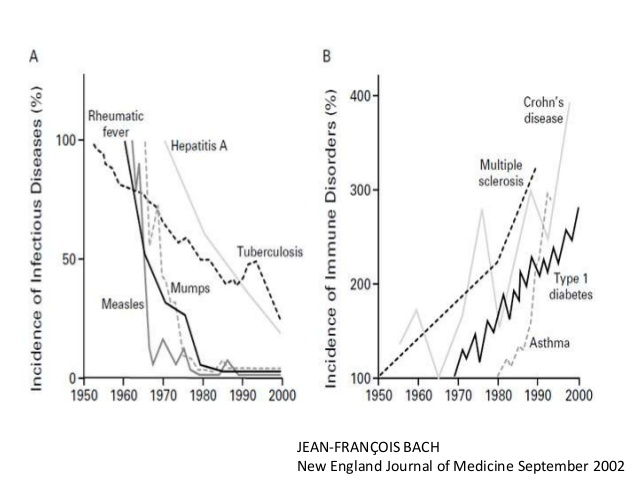
\includegraphics[scale=0.5]{img/allergie_infection.jpg}\hfill
\end{center}
\caption{Incidence des maladies infectieuses et auto-immunes en Europe au cours de 50 ans. }
\label{hyigienisme}
\end{figure}


Les méthodes récentes d'exploration de ce monde microscopique comme le séquençage haut-débit ont permis aux bactéries de retrouver leurs lettres de noblesse.
Elles sont présentes partout et jouent le premier rôle dans le fonctionnement des écosystèmes. Elles sont, par exemple, impliquées dans le cycle de l'azote et permettent à la biomasse d'absorber le diazote atmosphérique. Les bactéries sont ainsi la source primaire dans laquelle les organismes puisent pour construire leurs protéines et leurs acides nucléiques.
Elles peuvent survivre dans les milieux les plus inhospitaliers. Les archées (anciennement archéobactéries) peuvent résister dans des environnements d'acidité et de température exceptionnellement élevées ou faibles. On les retrouve dans les fonds océaniques où, privées de lumière, elles sont la seule source d'énergie pour la faune grâce à la chimiosynthèse à l'instar de la photosynthèse.
Le corps humain est lui aussi un environnement riche en bactéries. La majorité des bactéries a longtemps été indétectable par les méthodes de cultures classiques. Mais à présent, nous savons que les régions anatomiques autrefois considérées stériles contiennent beaucoup de bactéries.
On les retrouve sur tous les muqueuses et épithéliums du corps où elles se regroupent en communautés.
La peau est colonisée par \textit{Propionibacterium}, \textit{Corynebacterium} et \textit{Staphylococcus} \cite{Yong2017}. Le vagin est colonisé essentiellement par \textit{Lactobacillus} et la bouche principalement par \textit{Streptococcus}\cite{Yong2017}.
La muqueuse intestinale est colonisée par une « flore » bactérienne ou microbiote dominé par les anaérobies pouvant contribuer jusqu'à 0,2 kg au poids corporel \citep{Sender2016}.
En échange de notre hospitalité, le microbiote contribue au bon fonctionnement de son hôte. Il aide à la digestion en dégradant par exemple les sucres du lait maternel chez le nouveau-né \cite{Bode2012,Yong2017}. Il participe à la synthèse des vitamines essentielles (K, B12, B9)\cite{LeBlanc2013,Yong2017}. Il éduque notre système immunitaire et fait barrière à l'implantation de tout nouvel agent pathogène.
Tout déséquilibre du microbiote intestinal ou dysbiose peut avoir des conséquences pour notre santé. La liste des affections associées est longue \cite{Yong2017}. On y retrouve la maladie de Crohn, la maladie cœliaque, le cancer de l’intestin, le syndrome du côlon irritable, l’obésité, le diabète de type 1, l’asthme, l’eczéma, la sclérose en plaques, la polyarthrite rhumatoïde, la maladie d’Alzheimer et même l’autisme. \\
Par exemple, la destruction du microbiote intestinale par des antibiotiques donne l'opportunité à la souche toxinogène de \textit{Clostridium difficile} de s'installer et provoquer une colite pseudo-membraneuse. Un des traitements proposés après plusieurs échecs de traitement antibiotique est la transplantation fécale visant à régénérer le microbiote du patient. \\
Le microbiote nous amène donc à reconsidérer notre individualité. Nous ne sommes plus seulement un organisme multicellulaire composé d'un seul génome ; mais plutôt un écosystème où cellules eucaryotes et micro-organismes vivent en symbiose. Cette relation n'étant pas figée dans le temps et pouvant varier entre le commensalisme, le parasitisme et le mutualisme. Des études récentes ont permis d'estimer que pour un être humain le nombre de cellules microbiennes est de 39 milliards comparé aux 30 milliards de cellules humaines \cite{Sender2016}. En associant les gènes bactériens, le génome d’un être humain passe de 23 000  à 3,3 millions de gènes \cite{Qin2010} avec toute la complexité des interactions que cela engendre. Les scientifiques ont nommé \textit{holobionte} cet écosystème vivant. L'ensemble des génomes est appelé \textit{hologénome}. \\
Il faut toutefois rester prudent quant au rôle donné aux microbiotes et éviter de tomber dans l'excès. Nombreuses sont les publications scientifiques qui se contredisent ou qui confondent corrélation et causalité. Ces publications ont d'ailleurs conduit à la création du hashtag humoristique sur Twitter: \textit{\#GutMicrobiomeAndRandomSomething}.
Les études sur le microbiote doivent être étayées par des études fonctionnelles afin de trouver des relations de cause à effet. Les corrélations doivent être réalisées sur des populations plus grandes avec un suivi dans le temps plus conséquent. Les nouvelles technologies de séquençage haut-débit vont dans ce sens en collectant toujours plus de données.\\
Il est encore trop tôt pour dire si cette science va révolutionner la médecine ou s’il s'agit d'un effet de mode. Au regard de l'évolution biologique et de l'importance du microbiote chez d'autres espèces, les paris sont ouverts. Ne l'oublions pas, ce sont d'anciennes bactéries, que nous appelons aujourd'hui des mitochondries (Figure \ref{mitochondrie}), qui permettent à l'ensemble de nos cellules de respirer.

\begin{figure}[ht]
\begin{center}
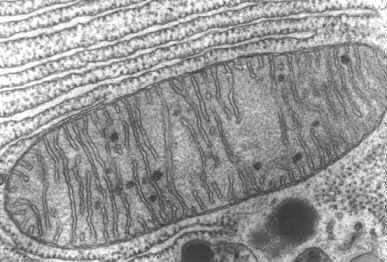
\includegraphics[scale=0.5]{img/mitochondrie.jpg}\hfill
\end{center}
\caption{La mitochondrie est l'exemple de symbiose ultime entre eucaryote et procaryote.}
\label{mitochondrie}
\end{figure}



\newpage

\section{Définitions}
\subsection{Termes utilisés en écologie}

\paragraph{Le microbiote\cite{Eisen}} est l’ensemble des micro-organismes (bactéries, levures, champignons, virus) vivant dans un environnement donné.
\paragraph{Le microbiome\cite{Eisen}} est l'ensemble des génomes du microbiote. Le plus souvent le microbiome fait référence aux génomes bactériens seuls. On parle alors de virome et de mycobiome pour les virus et champignons respectivement.

\paragraph{La biocénose} est le terme écologique dans un sens large désignant l'ensemble des organismes vivants dans un environnement appelé \textbf{biotope}. Biocénose et biotope forment ensemble un \textbf{écosystème}.

\paragraph{Une symbiose} est une association durable entre deux organismes. Leurs relations peuvent être mutualiste, parasitaire ou commensale.


\paragraph{L'OTU}(\textit{Operational Taxonomic Unit}) est un terme utilisé en phylogénie pour désigner un groupe d’individus semblables. Dans la majorité des cas, il s'agit de l'espèce dans la classification de Linné.
En microbiologie, un OTU est défini par un groupe de bactéries ayant une similarité dans leurs séquences d'ADNr 16S supérieur ou égal à 97 \%.

\paragraph{L'abondance} absolue est le nombre de reads d'un même OTU dans un échantillon. 
L’abondance relative est l'expression en pourcentage de l'abondance absolue. Cet indice est indirectement liée au nombre d'individu d'un même OTU constituant le microbiote.

\paragraph{La dominance} caractérise un OTU dont l'abondance est supérieure à 90 \% dans un échantillon.


\paragraph{La table des OTUs} est à la base de toute analyse en écologie. Elle correspond à un tableau à double entrée contenant l’abondance par échantillon et par OTU. Dans le tableau \ref{OTUTABLE}, l'abondance relative pour \textit{Staphylococcus aureus} est de 68 \%.

\begin{figure}[h]
\begin{center}
\begin{tabular}{|l|c|c|c|c}
  \hline
   & échantillon 1 & échantillon 2 & échantillon 3  \\
  \hline
  OTU 1 (\textit{S. aureus}) & 68 \% & 12 \% & 25 \% \\
  OTU 2 (\textit{E. coli})& 40 \% & 24 \% & 25 \% \\
  OTU 3 (\textit{P. aeruginosa}) & 28 \% & 64 \% & 50 \% \\

  \hline
\end{tabular}
\end{center}
\caption{La table des OTUs : l'abondance relative de 3 espèces bactériennes pour 3 échantillons}
\label{OTUTABLE}
\end{figure}

\paragraph{La diversité alpha} est une mesure de la biodiversité au sein d’un échantillon. Elle correspond à l'analyse d'une colonne de la table des OTUs. La richesse, l'indice de Chao1, de Shannon et de Simpson sont des indices de diversité alpha.

\paragraph{La diversité bêta} est une analyse descriptive de la biodiversité entre plusieurs échantillons. Elle correspond à l'analyse de l’ensemble de la table des OTUs. L’approche la plus courante est de réaliser une analyse multivariée par des méthodes d’ordination. Il s’agit de représenter un graphique à n dimensions, impossible à représenter dans toutes ses dimensions, en le projetant dans un espace à deux ou trois dimensions.

\paragraph{La richesse}(\textit{richness}) est le nombre d'OTUs présents dans un échantillon. Les deux échantillons suivants ont la même richesse (2), mais pas les mêmes abondances.

\begin{description}
\item[échantillon 1] : 4 \textit{Streptoccus}, 4 \textit{Escherichia}
\item[échantillon 2] : 432 \textit{Streptoccus}, 12 \textit{Escherichia}
\end{description}

\paragraph{L'équitabilité}(evenness) indique si les OTUs d’un échantillon sont répartis uniformément.
L'équitabilité du premier échantillon est plus grande que celle du second.

\begin{description}
\item[échantillon 1]  : 50 \textit{Streptococcus} , 50 \textit{Escherichia}
\item[échantillon 2]  : 432 \textit{Streptococcus}, 12 \textit{Escherichia}
\end{description}


\paragraph{L'indice Chao1}est une estimation de la richesse réelle (\textit{in vivo}) par rapport à la richesse observée dans l'échantillon (\textit{in vitro}). Cet indice part du principe que si l’échantillon contient beaucoup de singletons (OTU détecté une seule fois), il est fort probable que la richesse réelle soit plus grande que la richesse de l’échantillon. La formule est la suivante:

\begin{mycapequ}[!h]
   \begin{equation}
     Chao_{1} = S_{observed} + \frac{a^2}{2b}
   \end{equation}
      \caption{avec \textbf{S} la richesse observée, \textbf{a} le nombre de singletons et \textbf{b} le nombre de doubletons.}
\end{mycapequ}

\paragraph{L'indice de Shannon} est un indicateur évaluant à la fois la richesse et l'équitabilité dans un échantillon. Il se calcule de la même façon que l’entropie de Shannon.

\begin{mycapequ}[!h]
   \begin{equation}
     Shannon = \sum_{i=1}^Sp_{i}ln(p_{i})
   \end{equation}
      \caption{avec \textbf{p} la fréquence d'un OTU parmi les \textbf{S} OTUs présents dans l'échantillon.}
\end{mycapequ}

\paragraph{L'indice de Simpson}est un indicateur évaluant la probabilité que deux individus sélectionnés aléatoirement dans un échantillon donné soient de la même espèce. L'indice est de sens contraire aux précédents. La formule est la suivante:

\begin{mycapequ}[!h]
   \begin{equation}
     Simpson = 1 - \sum_{i=1}^Sp_{i}
   \end{equation}
      \caption{avec \textbf{p} la fréquence d'un OTU parmi les \textbf{S} OTUs présents dans l'échantillon}
\end{mycapequ}

\paragraph{La courbe de raréfaction}est utilisée pour déterminer si la profondeur de séquençage est suffisante pour caractériser la diversité d’un échantillon. Pour comprendre, imaginons un sac noir contenant des billes (reads) de différentes couleurs (espèces). Avec deux couleurs dans le sac, une petite poignée (un petit échantillon) de billes sera suffisante pour évaluer la diversité. Vous ne trouverez pas de nouvelle couleur avec plus de billes dans votre main. En revanche, avec d'avantage de couleurs dans le sac, il faudra une poignée plus importante pour évaluer la diversité. La courbe de raréfaction permet d'évaluer si cette poignée de billes est suffisamment représentative.
Pour générer cette courbe, des groupes de reads de taille croissante (1..n) sont tirés aléatoirement depuis l'échantillon. Le groupe est reporté sur l'axe X et le nombre d'OTUs trouvé dans ce groupe est reporté sur l’axe Y.
Une courbe s’aplatissant indique une bonne profondeur de séquençage (Figure \ref{rarefaction_demo}).


\begin{figure}[ht]
\begin{center}
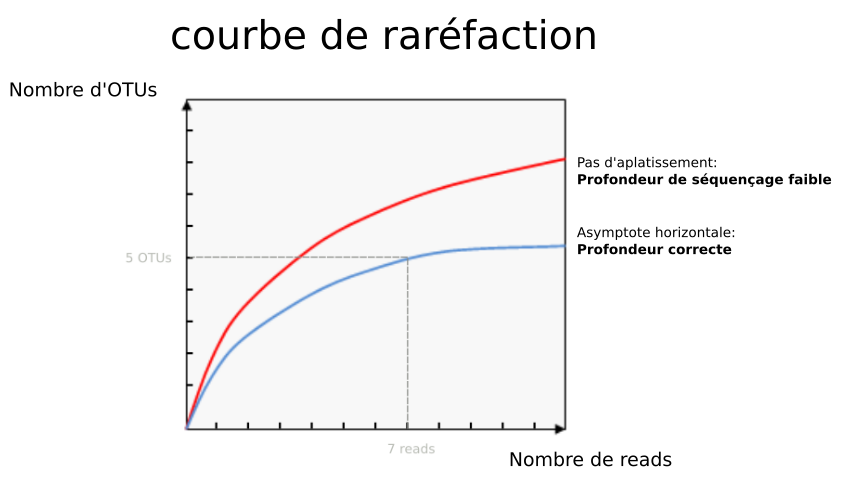
\includegraphics[scale=0.5]{img/rarefaction_example.png}\hfill
\end{center}
\caption{Exemple de courbes de raréfactions. La courbe bleue témoigne d'un bon échantillonnage en s’aplatissant précocement. Plus de reads ne permettraient pas de découvrir de nouveaux OTUs contrairement à la courbe rouge. }
\label{rarefaction_demo}
\end{figure}

\subsection{Termes utilisés en bio-informatique}

\paragraph{Un pipeline} est un ensemble d'étapes de calcul informatique. Chaque étape prend en entrée des fichiers pour en produire de nouveaux dans sa sortie. On peut comparer cela aux étapes d'une recette de cuisine. Sans parallélisation, un cuisinier (le processeur) doit attendre de faire fondre le beurre avant de battre les œufs en neige (exécution synchrone). En parallélisant, le cuisinier peut réaliser plusieurs étapes en même temps. Battre les œufs pendant que le beurre fond (exécution asynchrone).
Maintenant, si l'objectif est de produire 188 gâteaux (188 analyses) et que l'on dispose de 64 cuisiniers (64 processeurs), l'organisation des tâches devient complexe si l'on veut maximiser le rendement. Pour cela, on dispose d'outils comme \textit{Snakemake}\cite{Koster2012}, qui permettent de trouver la meilleure façon d'optimiser les tâches en construisant ce qu'on appelle un graphe orienté acyclique.

\paragraph{NGS}(Next Generation Sequencing) désigne l'ensemble des techniques de séquençage de nouvelle génération permettant de séquencer un nombre très important de fragments d'ADN.

\paragraph{La métagénomique} est une méthode d’étude du contenu en matériel génétique présent dans un milieu grâce aux techniques de séquençage haut débit. Contrairement à la génomique qui s’intéresse au génome d’un individu, la métagénomique s’intéresse aux génomes d’une population d’individus.
Dans son sens strict, la métagénomique correspond à l’étude de l’ensemble des séquences d'ADN. L’analyse d’un seul gène, comme celui de l’ARNr 16S est associé à tort au terme métagénomique, mais son usage reste courant. On lui préférera le terme de \textbf{métagénétique} ou \textbf{métataxonomique}.


\paragraph{Un \textit{read}} est un terme bio-informatique désignant une séquence d’ADN issue d’un séquençage haut débit. Selon les technologies, la longueur des reads varie le plus souvent entre 100 et 300 paires de bases.

\paragraph{Une librairie} est l'ensemble des fragments d'ADN préparés pour être séquencés.

\paragraph{Un score de qualité Phred} ou QScore exprime la confiance que l'on porte au séquençage. Il est lié de façon logarithmique à la probabilité d'erreur d'identification d'un nucléotide.  Par exemple un score de 10 équivaut à une 1 erreur sur 10. Un score de 40 à 1 erreur sur 10000.


\begin{mycapequ}[!h]
   \begin{equation}
    Q = -10 \ \log_{10} P
   \end{equation}
      \caption{Le score Q est associé de façon logarithmique à la probabilité d'erreur P de s'être trompé en séquençant un nucléotide.}
\end{mycapequ}




\paragraph{Une ordination} est une analyse multivariée visant à décrire des objets caractérisés par plusieurs variables. Par exemple un échantillon est caractérisé par différentes abondances de bactéries. Il existe plusieurs méthodes d'ordination. La plus connue étant l'Analyse en Composantes Principales (PCA) basée sur une matrice de covariances. En écologie l'Analyse en Coordonnées Principales (PCoA) est préférée. Elle se base sur une matrice de distances. Elle consiste à projeter des points d'un espace à n dimensions vers un espace visible en 2 dimensions.
La figure \ref{pcoatuto} illustre ce principe avec un exemple à deux dimensions seulement.

\begin{figure}[!h]
\begin{center}
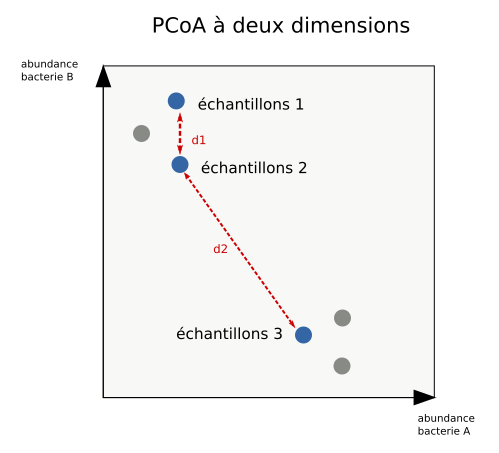
\includegraphics[scale=0.6]{img/pcoatuto.png}\hfill
\end{center}
\caption{Représentation graphique d'une analyse en coordonnées principales (PCoA) de plusieurs échantillons ne contenant que deux espèces A et B. Chaque échantillon est assimilable à un point de coordonnées (abondance A; abondance B). Il est alors possible de calculer des distances entre les échantillons. La plus connue étant la distance euclidienne. Mais d'autres existent comme la distance de Bray-Curtis. Sur cette figure, les échantillons 1 et 2 ont des microbiotes proches, car la distance d1 qui les sépare est petite. Dans la réalité, il y a plus d'espèces donc plus de dimensions. Une PCoA consiste à réduire cet espace multidimensionnel en un espace 2D qui respecte les distances entre les points. }
\label{pcoatuto}
\end{figure}
\newpage

\paragraph{La distance de Bray-Curtis} est un indice de dissimilarité entre deux échantillons qui s'assimile à une distance entre 2 points dans un espace de taille n (Figure \ref{pcoatuto}). Plus la distance est grande et plus les deux échantillons sont dissemblables. La formule est la suivante :

\begin{mycapequ}[!h]
   \begin{equation}
    BC_{jk} = 1 - \frac{2\sum_{i=1}^{p}min(N_{ij},N_{ik})}{\sum_{i=1}^{p}(N_{ij} + N_{ik})}
   \end{equation}
      \caption{Où $N_{ij}$ est l'abondance d'une  espèce i dans l'échantillon j et $N_{ik}$ l'abondance de la même espèce i dans l'échantillon k. Le terme min(.,.) correspond au minimum obtenu pour deux comptes sur les mêmes échantillons. Les sommes situées au numérateur et dénominateur sont réalisées sur l'ensemble des espèces présentes dans les échantillons.}
\end{mycapequ}


\paragraph{Un fichier fastq} contient les séquences des reads et leurs qualités par nucléotides exprimés en Phred Score. Chaque read est représenté par 4 lignes dans un fichier textuel (Figure \ref{fastq}). Ces fichiers sont produit par le séquençage haut-débit.

\begin{figure}[!h]
\begin{center}
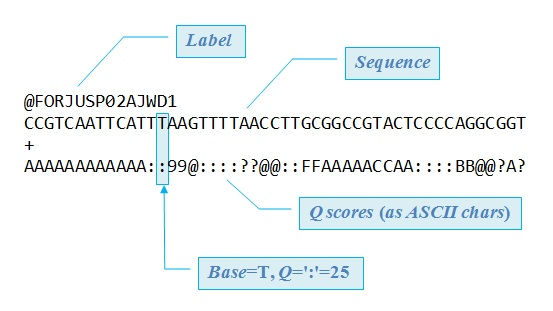
\includegraphics[scale=0.6]{img/fastq.jpg}\hfill
\end{center}
\caption{Exemple d'un read contenu dans un fichier FASTQ. Les scores de qualités sont encodés avec des symboles ASCII. Par exemple le quatorzième T  est associé au symbole « : » correspondant au score phred de 25, soit une probabilité de 0,3 \% d'erreur.}
\label{fastq}
\end{figure}

\paragraph{Le multiplexage} est utilisé pour pouvoir séquencer plusieurs échantillons différents dans une même librairie. Pour cela, les ADNs de chaque échantillon sont marqués avec une courte séquence nucléotidique appelée barcode ou index suivant la technologie. Lors de l'analyse bio-informatique, les données sont démultiplexées afin d'associer chaque read à son échantillon.

\paragraph{Un graphe} est un objet mathématique défini par des nœuds (nodes) reliés par des arrêtes (edges). Les graphes permettent de répondre à différents problèmes mathématiques. Par exemple, le problème des sept ponts de Königsberg, qui consiste à savoir s'il existe une promenade passant par 7 ponts une seule fois. La théorie des graphes est très utilisée en bio-informatique.

\newpage

\setcounter{page}{1}

\section{Introduction}
\subsection{La mucoviscidose}
\subsubsection{Une maladie génétique}
La mucoviscidose est une maladie génétique autosomique récessive grave qui touche en France 1 naissance sur 5400\cite{Registredelamuco.org}. La Bretagne est la région la plus touchée avec une prévalence de 1/3000\cite{Registredelamuco.org}.
La loi de Hardy Weinberg estime qu’en Bretagne, 1 personne sur 27 est porteuse d'une mutation dans /textit{CFTR} à l’état hétérozygote. Cette haute prévalence s’explique probablement par un effet fondateur associé à un avantage sélectif pour les individus porteurs de l’allèle muté\footnote{Plusieurs hypothèses ont été proposées, notamment celle de la diminution des pertes hydriques chez les sujets hétérozygotes lors des grandes épidémies de choléra.}.
Le gène \textit{CFTR} impacté se situe sur le chromosome 7 en position q31.2. Il est constitué de 27 exons pour 250 188\cite{OLeary2016} paires de bases. Il code un canal chlore AMP dépendant permettant les échanges des ions chlorures au niveau des membranes cellulaires. Il est également impliqué dans le transport du thiocynate (SCN-) et des bicarbonates (HCO3-)\cite{Quinton2001}.
On dénombre à ce jour 2017 mutations \cite{cftrdb} mises en cause dans la mucoviscidose. La perte d’une phénylalanine en position 508 par délétion de trois nucléotides c.1521-1523delCTT (anciennement $\Delta$F508) cause à elle seule 80 \% des mucoviscidoses\cite{cftrdb}.
Ces mutations sont responsables d’une protéine défectueuse ou d’une absence de canaux sur les membranes cellulaires. \\
Cliniquement, la mutation entraîne une insuffisance pancréatique exocrine et une infertilité par disparition des canaux déférents. Des signes digestifs, hépatiques et articulaires sont également présents.
L'atteinte de la fonction respiratoire est la plus bruyante cliniquement. En effet, au niveau de l’épithélium broncho-pulmonaire, l’absence d’une protéine CFTR fonctionnelle est responsable d’une déshydratation du mucus le rendant plus visqueux et empêchant les cils bronchiques de jouer leurs rôles.\\
La forte prévalence de la maladie nécessite de réaliser un dépistage précoce chez tous les nouveaux-nés (test de Gutri) afin d’adapter au plus tôt la prise en charge. Le test à la sueur est la méthode diagnostique de référence. Le dépistage prénatal basé sur l’ADN circulant est actuellement à l’étude\cite{Guissart2017}.\\
Le traitement repose avant tout sur une prise en charge respiratoire (kinésithérapie, dornase \footnote{Une DNase qui fluidifie les sécrétions trop riches en ADN provenant de l'afflux des neutrophiles in situ et de leur apoptose prématurée.}, antibiothérapie). Les recherches en thérapie génétique sont encourageantes \cite{Montier2004}.
Les traitements correcteurs/potentiateurs de la protéine CFTR, comme l'\textit{ivacaftor} sont les seuls traitements curateurs, mais concernent uniquement certaines mutations rares comme la G551D. La greffe pulmonaire est le dernier recours.

\subsubsection{Une maladie infectieuse et inflammatoire}

L’atteinte pulmonaire dans la mucoviscidose est caractérisée par des réactions inflammatoires qui dégradent progressivement la fonction respiratoire. Cette inflammation est la conséquence d'un afflux excessif de polynucléaires avec libération de médiateurs\cite{Heijerman2005} probablement en réponse à une agression microbienne. Plusieurs pathogènes sont impliqués. Chez les jeunes enfants\cite{Davies}, \textit{Haemophilus influenzae} et \textit{Staphylococcus aureus} sont le plus souvent responsable. \textit{Achromobacter xylosoxidans}, \textit{Burkholderia cepacia complex} et \textit{Stenotrophomonas maltophilia} sont retrouvés parmi les sujets plus âgés \cite{Davies}.

Mais c’est \textit{Pseudomonas aeruginosa} qui caractérise l’atteinte pulmonaire dans la mucoviscidose en marquant un tournant décisif dans l’évolution de la maladie. Ce bacille aérobie strict est une bactérie de l'environnement rarement retrouvée parmi les sujets sains\cite{Plesiat}. En revanche, dans la mucoviscidose, il est mis en évidence\cite{LeBourgeois} chez 60 \% des patients jeunes et chez plus de 90 \% des patients adultes.\\
La primocolonisation à \textit{P. aeruginosa} semble avoir lieu tôt dans l’enfance[@]. Il y a ensuite une phase de latence, variable entre les individus, marquée par des épisodes de recolonisation intermittentes. À ce moment, l’éradication par des antibiotiques reste possible.
Puis survient le passage à la chronicité. \textit{P. aeruginosa} s'adapte à son milieu et s’installe à long terme. Il perd certains caractères de virulence, mais devient résistant aux antibiotiques\cite{LeBourgeois}. Son phénotype change. Il se transforme pour devenir mucoïde en sécrétant un film d’alginate qui le protège du système immunitaire. Les mécanismes sous-jacents à cette adaptation sont ingénieux. La forte densité en bactéries est responsable de l’activation de certains gènes par un processus appelé \textit{quorum sensing}\cite{Ruimy2004}. Dans ce processus, chaque bactérie communique avec ses voisines par des signaux chimiques.

Le génome de \textit{Pseudomnas aeruginosa} devient aussi hyperpermutable\cite{Davies} pour présenter une plus grande diversité génétique au regard de la sélection naturelle\footnote{En biologie évolutive, il s'agit d'évolvabilité} et donc évoluer plus rapidement. \\
À ce stade, le traitement antibiotique n’est plus curatif mais symptomatique et l'évolution tend inexorablement vers un déclin de la fonction respiratoire. \\
L'approche clinique est donc préventive afin de retarder le passage à la chronicité. Elle vise à éliminer \textit{Pseudomnas aeruginosa} dès qu'il est détecté en culture grâce à une surveillance rapprochée \cite{LeBourgeois}. La culture étant peu sensible, d’autres méthodes d'identification peuvent être employées. La détection des anticorps anti-pyocyaniques par ELISA a montré peu de sensibilité et n'est plus recommandée à l'heure actuelle \cite{Plesiat}.
La PCR ciblée associant les gènes des protéines bactériennes \textit{oprL}, \textit{gyrB} et \textit{ecfX} s’est montrée plus sensible et plus spécifique que la culture\cite{LeGall}. \\
En pratique, la colonisation chronique est définie lorsque 3 expectorations sont rendues positives en culture, successivement au cours d’un suivi mensuel ou bimensuel \cite{LeBourgeois}.
Une autre classification, celle de Lee\cite{Lee2003} définit 4 groupes (Tableau \ref{lee}):

 \begin{table}[h]
     \centering
     \caption{Classification de Lee \cite{Lee2003}}
     \begin{tabular}{|c|p{10cm}|}
      \hline
          \textbf{chronique} & > 50 \% des cultures sont positives sur 12 mois \\
         \hline
         \textbf{intermédiaire} & $\leq$ 50 \% des cultures sont positives sur  12 mois\\
          \hline
          \textbf{Free} & Cultures nég. sur 12 mois avec des antécédents de positivité à \textit{P. aeruginosa}\\
         \hline
	    \textbf{Never} & Cultures nég. sur 12 mois sans antécédents de positivité à \textit{P. aeruginosa} \\
	      \hline
     \end{tabular}
     \label{lee}
 \end{table}


A ce jour, la physiopathologie de l'infection broncho-pulmonaire chez les patients atteints de mucoviscidose est encore mal comprise ; Par exemple, on ne sait pas clairement pourquoi \textit{Pseudomnas aeruginosa} s’installe préférentiellement chez les patients atteints de mucoviscidose. Plusieurs hypothèses ont été proposées:

\textbf{Déshydratation du mucus}\cite{Davies}:
La mutation \textit{CFTR} serait responsable d'un mucus plus visqueux et moins épais associé à une la perte de fonction des cils bronchiques. Les bactéries seraient alors piégées dans ce mucus pour être exposées plus longtemps à l'épithélium respiratoire et ainsi déclencher une réponse inflammatoire.

\textbf{Augmentation de salinité}\cite{Davies}:
L'augmentation de la salinité du mucus aurait pour conséquence de désactiver des peptites antimicrobiens présents comme les bêta-defensines, lysozymes ou les lactoferrines.

\textbf{Adhérence aux cellules}\cite{Davies}:
\textit{P. aeruginosa} serait un ligand naturel des cellules épithéliales portant la protéine CFTR non mutée. Après internalisation, la bactérie serait détruite.

\textbf{Création d'un milieu favorable}:
L'inflammation précède la colonisation à \textit{P.aeruginosa} et crée un milieu favorable.
Par exemple la production d'alanine et de lactate \cite{Boulette2009} est une source de carbone métabolisable par \textit{P. aeruginosa}.

\textbf{Stimulation du système immunitaire}:
\textit{P. aeruginosa} stimulerait le système immunitaire de façon à éliminer tous ses concurrents et ainsi se développer seul dans sa niche écologique.

\textbf{Une anomalie du microbiote \cite{HoMan2017}}:
A l'instar de ce qui est bien démontré au niveau intestinal, le microbiote respiratoire jouerait le rôle de barrière contre l'implantation d'agents pathogènes exogènes. La dysbiose induite par la mucoviscidose permettrait à \textit{P.aeruginosa} de s'installer (Keravec et al., 2015).


\begin{figure}[ht]
\begin{center}
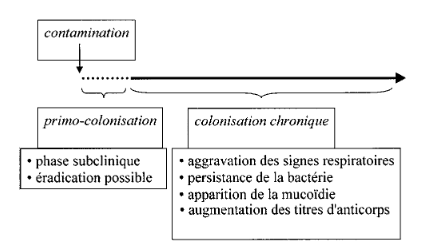
\includegraphics[scale=0.8]{img/chronic.png}\hfill
\end{center}
\caption{Histoire naturelle de l'infection pulmonaire à \textit{P. aeruginosa} dans la mucoviscidose (P.Plésiat 2003\cite{Plesiat}).}
\label{bach}
\end{figure}


\subsection{Le microbiote pulmonaire}

Bien qu'il soit en contact avec le milieu extérieur, l’arbre respiratoire (comprenant la trachée, les bronches et les alvéoles) a longtemps été considéré stérile avec les méthodes de culture classique. Il a fallu attendre l’avènement du séquençage haut débit pour mettre en évidence le microbiote pulmonaire \cite{HoMan2017,Beck,Dicksonb}.\\
L'arbre respiratoire chez le fœtus\footnote{Un article récent critique l'idée d'un fœtus stérile \cite{Perez-Munoz2017}} est stérile. Il se colonise comme l'intestin, à la naissance lors du passage de la filière génitale puis se différencie au cours du temps. Il est beaucoup moins riche que le microbiote digestif, mais plus dynamique en raison d'un flux aérien bidirectionnel.  Les bactéries du microbiote respiratoire proviennent de l’air ambiant, des voies supérieures, mais aussi du tube digestif par un phénomène de micro aspirations \cite{Dickson}. Une étude a d'ailleurs montré une concordance entre le microbiote digestif et respiratoire\cite{Dickson}.\\
Le microbiote pulmonaire est dominé par le phylum des \textit{Firmicutes} (\textit{Streptococcus}) et des \textit{Bacteroidetes} (\textit{Prevotella}). Les genres retrouvés majoritairement sont \textit{Streptococcus}, \textit{Prevotella}, \textit{Fusobacteria}, \textit{Veillonella}, \textit{Haemophilus}, \textit{Neisseria} et \textit{Porphyromonas}.
L’arbre respiratoire étant en continuité directe avec les voies aériennes supérieures, certains genres bactériens sont communs, comme \textit{Streptococcus}, \textit{Staphylococcus}, \textit{Haemophilus} et \textit{Moraxella}. Tandis que d’autres genres comme \textit{Corynebacterium} et \textit{Dolosigranulum} ne sont retrouvés qu’au niveau du nez et de l'oropharynx. \\
Le microbiote pulmonaire est dynamique. Il peut varier dans l'espace à cause de la structure irrégulière de l'arbre bronchique. Un prélèvement au niveau d'un foyer infectieux, par exemple, se distinguera nécessairement d'un foyer sain. Il existe également des gradients physico-chimiques qui selon la région peuvent sélectionner des espèces. Les cavernes tuberculeuses par exemple se trouvent essentiellement dans le lobe supérieur en raison d'une concentration en oxygène plus élevée qui favorise ce bacille aérobie strict. D'autres études \cite{Frayman2017,Coburn2015} ont montré que la diversité diminue avec l'âge ou encore que la structure du microbiote change avec une exposition tabagique.
Enfin, les pathologies respiratoires\cite{HoMan2017} sont une autre source de variabilité du microbiote. Il est par exemple démontré dans la mucoviscidose qu'il y une augmentation de richesse et une diminution de diversité. L'asthme et la BPCO sont également associés à des anomalies du microbiote pulmonaire\cite{Dicksona,Nguyen2015}.  \\
Il semble cependant que ce soit l'individu lui-même qui soit la principale source de variabilité avant tout autre facteur\cite{Whelan2017}. C'est-à-dire que l'environnement et le génome d'un individu sont les principaux déterminants du microbiote pulmonaire.

\subsection{Exploration du microbiote pulmonaire}
%(http://bacterioweb.univ-fcomte.fr/bibliotheque/remic/08-Bronc.pdf) ==> A LIRE COOURS BACTERIO

\subsubsection{Méthodes de prélèvement}
Le microbiote respiratoire est exploré en séquençant l'ADN des micro-organismes présents dans un échantillon.
Toutes les méthodes de recueil sont possibles, mais les prélèvements protégés (combicath, Liquide Broncho Alvéolaire (LBA)) sont recommandés afin
d’éviter une contamination par les voies aériennes supérieures. En pratique, les patients atteints de mucoviscidose sont suivis par le recueil des prélèvements moins invasifs comme les prélèvements pharyngés ou les expectorations spontanées ou induites (ECBC, examen cytobactériologique du crachat). Dans ces dernières, la qualité du prélèvement peut être évaluée en comptant le nombre de cellules épithélium (normalement < 25 par champ à l'objectif x10) et de polynucléaire (normalement > 10 par champ à l'objectif x10) selon le score de Bartlett adapté par Murray et Washington (REMIC 2015). Des prélèvements sont également réalisables \textit{in situ}  sur les explants lors des greffes pulmonaires.

\subsubsection{Séquençage haut débit}
% Baisse du coup du sequencage ... %
Le séquençage de nouvelle génération permet de séquencer de grandes quantités d'ADN dans un échantillon et ainsi de déterminer sa composition en bactéries ou autres micro-organismes. À titre d'exemple, un séquenceur Sanger classique permet de lire des fragments d'ADN d'environ 800 pb parallélisable jusqu'à 96 fois en augmentant le nombre de capillaires.
À l'inverse, un séquenceur de nouvelle génération lit des fragments plus courts de l'ordre de 150 pb. Mais la parallélisation peut aller jusqu'à 20 milliards de fois en un seul run sur un Illumina Novaseq. \\
Deux stratégies de séquençages sont utilisées en écologie microbienne:  \\
\textbf{La stratégie shotgun} consiste à séquencer l'ensemble des  ADN présents dans l'échantillon sans discernement, qu'ils soient humains ou bactériens. Les séquences sont filtrées puis les génomes bactériens sont reconstruits par des méthodes bio-informatiques complexes. \\
\textbf{La stratégie Amplicon} est moins coûteuse sur le plan de l'analyse. Elle consiste à séquencer un gène spécifiquement bactérien et suffisamment variable pour discriminer une espèce. Il s'agit du gène de l'ARNr 16S.\\
L'ARNr 16S est un ARN non codant participant à la structure de la petite sous unité des ribosomes bactériens. Il est composé de 1542 nucléotides et forme plusieurs boucles dans sa structure secondaire (Figure \ref{ARN16S}).
L'alignement des séquences d'ADNr 16S entre plusieurs espèces met en évidence des régions constantes et 9 régions variables (Figure \ref{ARN16SVariation}). Les régions constantes permettent de concevoir des amorces s'hybridant sur tous les ADNs bactériens. Les régions variables apportent la spécificité taxonomique permettant d'identifier l'espèce bactérienne.
% Les études de [@] ont montré que certaines régions variables apportent plus de spécificité.

\begin{figure}[ht]
\begin{center}
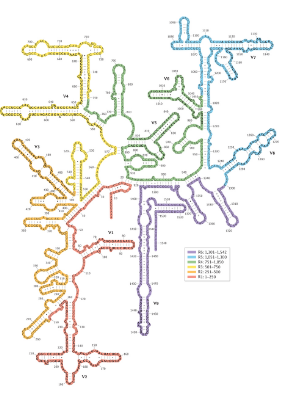
\includegraphics[scale=0.8]{img/ARN_16S.png}\hfill
\end{center}
\caption{Structure secondaire de l'ARNr 16S}
\label{ARN16S}
\end{figure}

\begin{figure}[ht]
\begin{center}
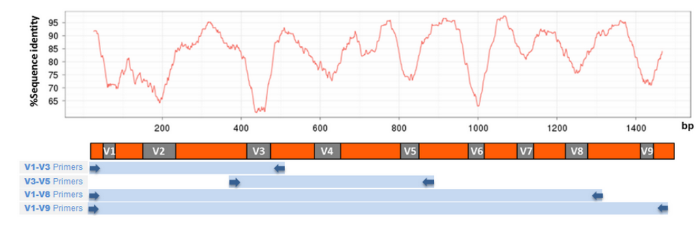
\includegraphics[scale=0.8]{img/ARN16S_variation.png}\hfill
\end{center}
\caption{Régions constantes et variables de l'ADNr 16S}
\label{ARN16SVariation}
\end{figure}

En séquençant l'ensemble des génomes bactériens, la stratégie \textit{shotgun} est plus informative, car elle permet de prédire la fonction d'un microbiote. En effet, les transferts génétiques horizontaux amènent à dissocier l'espèce de sa fonction. Deux bactéries d'une même espèce peuvent avoir des fonctions différentes. L'inférence fonctionnelle à partir de la deuxième stratégie est possible, mais déconseillée.
La stratégie 16S reste toutefois une méthode simple pour décrire les populations bactériennes présentes. C'est cette stratégie qui a été utilisée dans notre étude.



\subsection{Objectif de l'étude Mucobiome}
L'objectif principal de l'étude MUCOBIOME est de déterminer si dans la mucoviscidose, le microbiote respiratoire influence la colonisation à \textit{P. aeruginosa}.
Pour cela, nous avons suivi pendant 3 ans,  une cohorte de 97 patients atteints de mucoviscidose exempts de \textit{P. aeruginosa} depuis au moins 1 an.
L'exploration de leur microbiote par la stratégie 16S a été réalisée à partir d'expectorations bronchiques obtenues dans le cadre de leur suivi longitudinal.
À partir des données générées par le séquençage, nous avons effectué l'étude descriptive et analytique de leur microbiote en créant un pipeline bio-informatique dédié. L'objectif principal de ce travail de thèse a été la mise au point et l'évaluation de ce pipeline créé à façon pour l'étude MUCOBIOME.

\section{Matériel et Méthodes}
\subsection{Recueil des données}

Quatre-vingt-dix-sept patients atteints de mucoviscidose ont été suivis sur 3 ans (2008-2011) dans une étude prospective multicentrique (Nantes, Brest, Roscoff) appelée \textit{Mucobiome}.
Le comité de protection des personnes (CPP VI-Ouest) et le comité d’éthique du CHRU de Brest ont approuvé le protocole. Tous les patients (ou les parents pour les mineurs) ont signé un consentement éclairé. Le protocole a fait l’objet d’une déclaration de biocollection à l’ARS et au MESR (n° DC-2008-214).\\
Les expectorations des patients ont été recueillies lors des séances de kinésithérapie respiratoire, tous les 3 mois selon le calendrier des recommandations officielles. En pratique, sur l’ensemble de la cohorte suivie, l’intervalle médian entre 2 consultations a été de 3,4 mois.
Les patients devaient avoir un génotypage \textit{CFTR} et un test à la sueur positif. Les transplantés pulmonaires ont été exclus de l’étude.
Pour être inclus, le patient devait être exempt de \textit{P. aeruginosa} depuis au moins un an d’après les résultats de la culture bactérienne des expectorations. Le patient devait être en capacité d’expectorer spontanément (exclusion des prélèvements pharyngés).
La première culture bactérienne positive à \textit{P. aeruginosa} était le « endpoint » de l’étude. À cette étape, le patient était sorti de l’étude pour être réinclus un an plus tard en cas de maintien de la négativité des cultures bactériennes obtenue par l’antibiothérapie d’éradication anti-\textit{P. aeruginosa}. D’autres données clinico-biologiques* ont également été recueillies. Au total, 756 expectorations ont été recueillies à l’issue de l’étude MUCOBIOME. Pour ce travail portant sur l’étude du microbiote broncho-pulmonaire, 188 ont été sélectionnées dont 22 expectorations positives à \textit{P. aeruginosa}.

*citer qq exemples de données (que tu exploiteras après) et préciser le score
cytologique (à mettre dans les résultats : impact oui ou non sur les données du microbiote)

\begin{table}[h]
\centering
   \caption{démographie}
   \begin{tabular}{|l|c|c}
        \hline
   \multicolumn{3}{|c|}{     57 patients     } \\
    \hline
    age & \multicolumn{2}{|c|}{34}  \\
    \hline

        & 2.2 & 2.3 \\
    \hline
   \end{tabular}
\end{table}

\subsection{Extraction de l’ADN}

La procédure d'extraction des ADN des échantillons est détaillée dans la publication de  F. Gall\cite{LeGall}. Brièvement les échantillons ont été liquéfiés avec du Dithiotréitol (DTT). Les protéines ont été dégradées avec de la protéinase K.
Les parois bactériennes ont été fragmentées par sonication (DTT par sonication, Elamsonic S10, Singen, Germany). Après 10 min de centrifugation, L’ADN a été extrait à partir du culot à l'aide du kit QUIAamp DNA Minikit (Quagen).
Les extraits d’ADN ont été envoyés pour séquençage par le prestataire GATC.

\subsection{Séquençage}
La librairie a été générée en amplifiant la région V3-V5 à l’aide du couple d’amorces forward CCTACGGGAGGCAGCAG et reverse CCGTCAATTCMTTTRAGT et du kit MiSeq Reagent Kits v3. \\
Le séquençage a été réalisé sur Illumina MiSeq pour produire un couple de séquences chevauchantes de 300 pb (Figure \ref{illumina}). Après fusion du couple, le séquençage permet de lire  535 pb correspondant à la région V3-V5.\\
Environ 25 millions de reads sont produits par run MiSeq. En multiplexant à l’aide de 94 indexes, les 188 échantillons ont été séquencés sur 2 runs pour produire 188 x 2 fichiers fastq.

\begin{figure}[ht]
\begin{center}
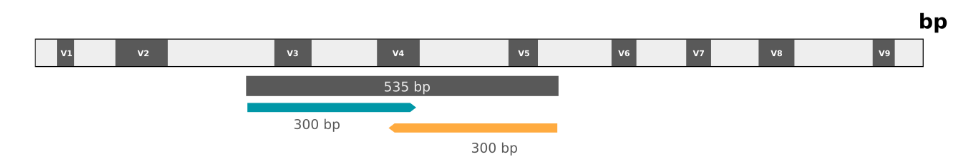
\includegraphics[scale=0.6]{img/illumina.png}\hfill
\end{center}
\caption{le couple de séquence de 300 pb permet de recouvrir l'ensemble de la région V3-V5 de l'ARN 16S}
\label{illumina}
\end{figure}


\subsection{Analyse bio-informatique}
L’analyse des 188 paires de fichiers fastq a été réalisée grâce à un pipeline bio-informatique, appelé \textit{mucobiome}, conçu et testé dans le cadre de cette étude. Par rapport aux autres logiciels comme \textit{QIIME}\cite{Caporaso2010} ou \textit{MOTHUR}\cite{Schloss2009}, le pipeline mucobiome est spécialisé dans l’analyse des données 16S. Il est également plus rapide en raison d’un très haut niveau de parallélisation permis grâce à  \textit{Snakemake}\cite{Koster2012}. Cet outil modélise l'ensemble du pipeline sous forme d'un graphe direct acyclique (DAG) et le résout afin d'optimiser la parallélisation. \\
Le pipeline mucobiome prend en entrée, les 188 couples de fichiers FASTQ provenant du séquençage et produit un fichier BIOM contenant la table des OTUs. Les figures \ref{pipeline_trio} et \ref{dag} illustrent toutes les étapes du pipeline qui sont décrites ci-dessous.



\begin{figure}[!ht]
\begin{center}
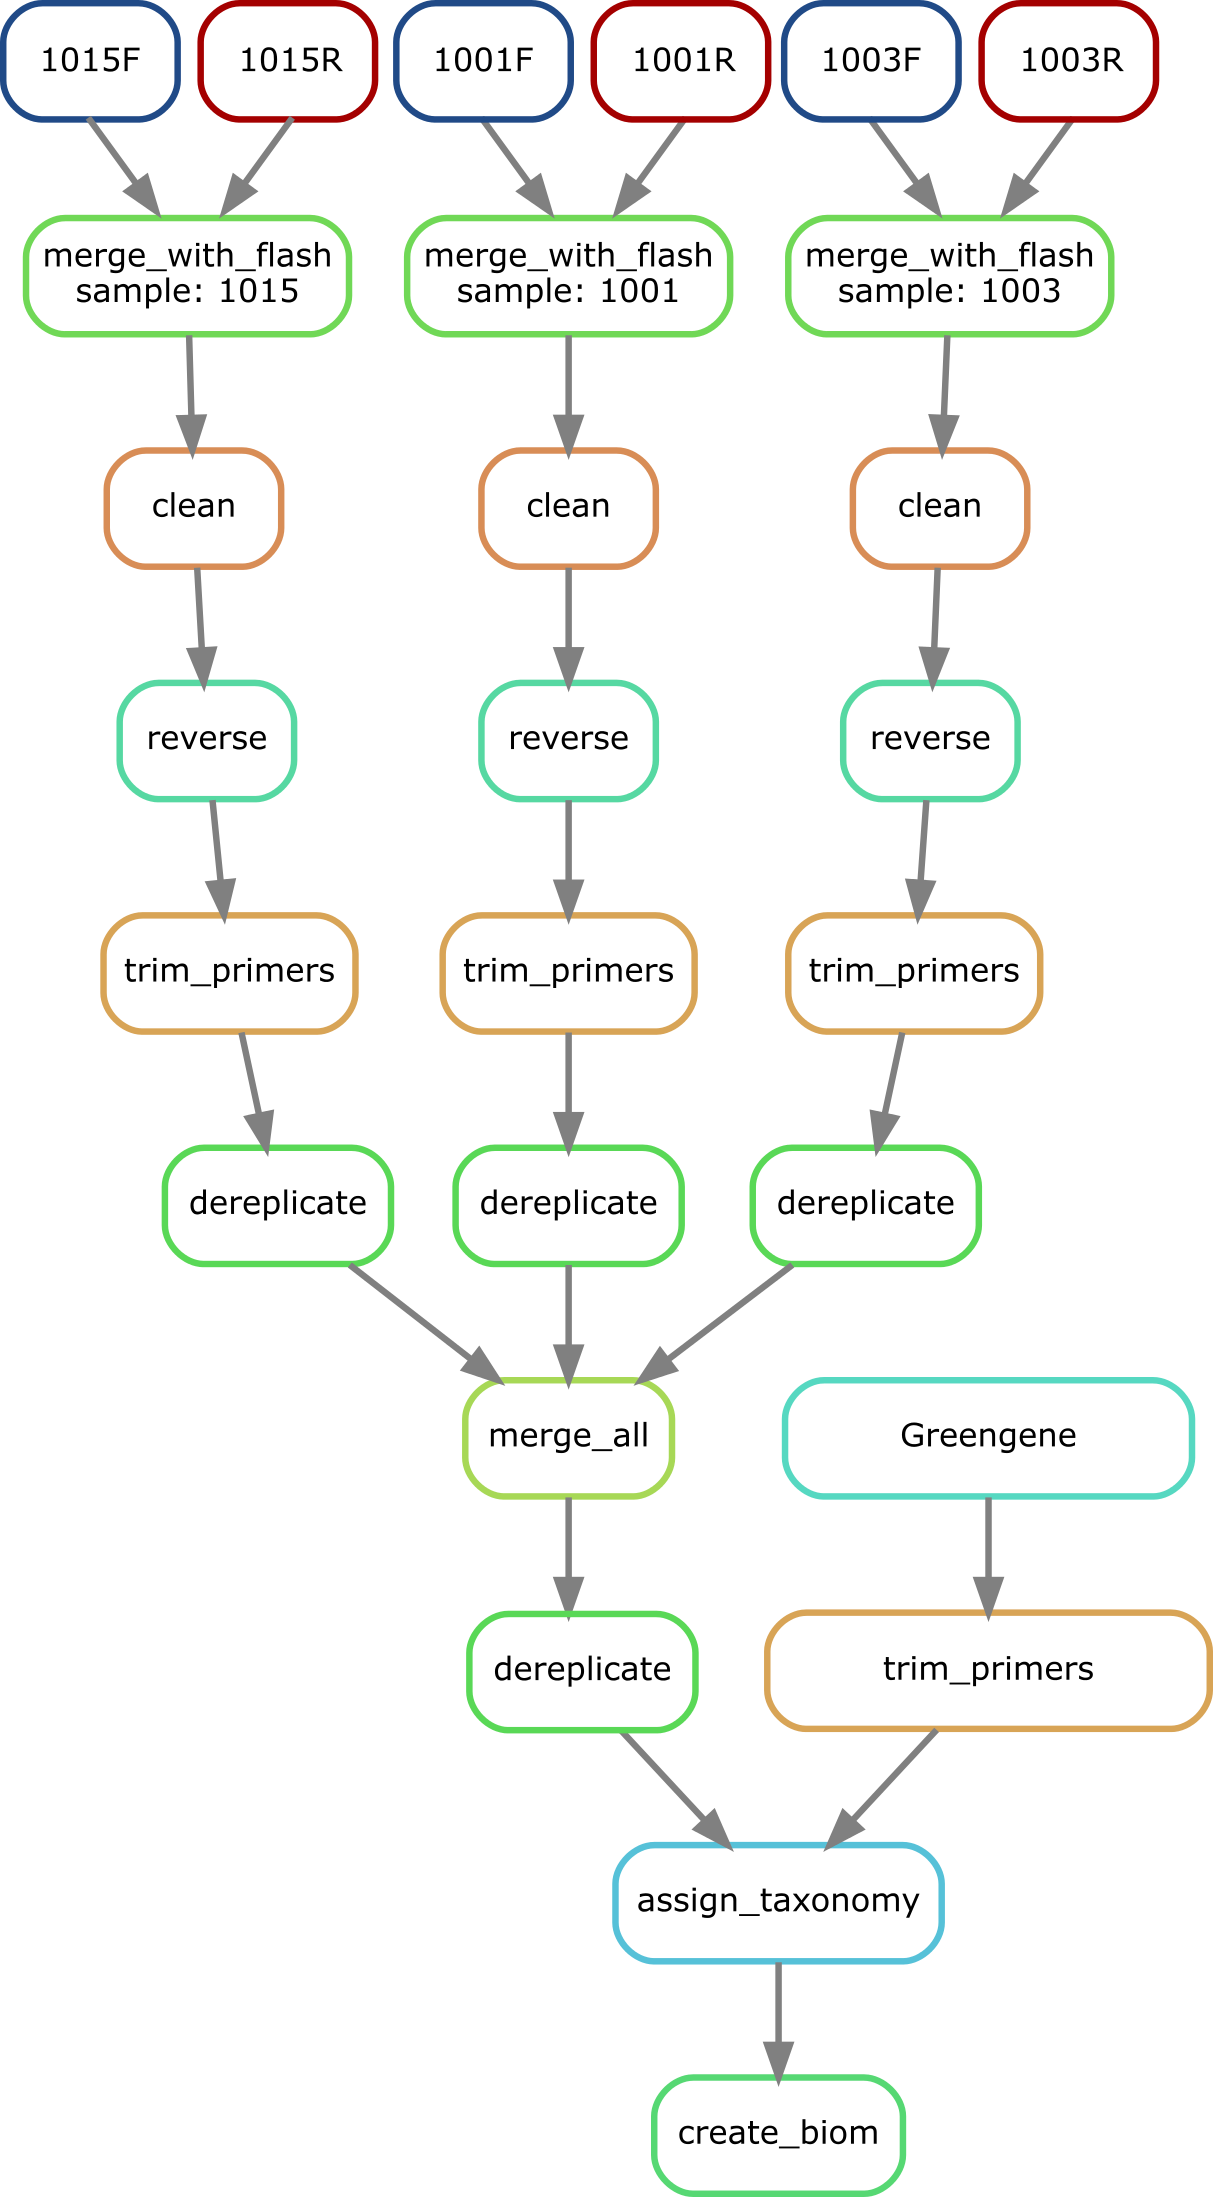
\includegraphics[scale=0.5]{img/pipeline_trio.png}\hfill
\end{center}
\caption{Graphe du pipeline simplifié sur 3 échantillons (1015, 1001 et 1003).\\ \textbf{Merging}: Les reads pairs de 300 pb sont fusionnés  pour produire un fichier fastq contenant des reads de 535 pb. \textbf{Cleaning}: Les reads de mauvaise qualité sont supprimés. \textbf{Reversing}: Les reads sont transformés en leurs séquences complémentaires pour pouvoir être alignés. \textbf{Trimming}: Seule la séquence entre les primers V3-V5 est conservée. \textbf{Dereplicating}: Les séquences dupliquées sont retirées. \textbf{Merging}: L'ensemble des séquences est regroupé dans un seul fichier. \textbf{Taxonomy assignement}: Les séquences sont alignées sur la base de données \textit{Greengene}. \textbf{create\_biom}: la table des OTUs est créée }
\label{pipeline_trio}
\end{figure}


\begin{figure}[ht]
\begin{center}
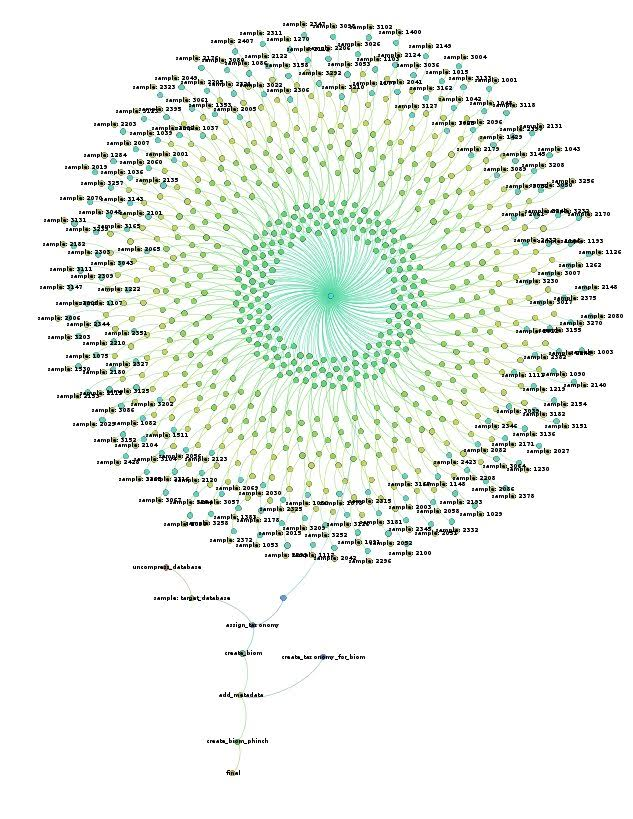
\includegraphics[scale=0.4]{img/dag.jpg}\hfill
\end{center}
\caption{le graphe du pipeline sur l'ensemble des échantillons. Le tournesol montre le niveau de parallélisation nécessaire.}
\label{dag}
\end{figure}

\subsection{Étape du pipeline}
\subsubsection{Merging: Fusions des reads}
\noindent\emph{ 2 fastq en entrée 1 fastq en sortie. }

La première étape du pipeline consiste à fusionner le couple de fichiers fastq afin de produire un seul fichier contenant des plus longues séquences de 535 pb correspondant à la région V3-V5 de l’ARNr 16S.
Le programme \textbf{Flash}\cite{Mago2011} a été utilisé avec les paramètres par défaut. À partir de deux fichiers fastq, ce dernier recherche le meilleur alignement entre deux reads et produit un fichier fastq contenant les reads fusionnés.
Une analyse qualitative des reads a été réalisée avec \textbf{FastQt}\citep{Labsquareteam2017} avant et après fusion.

\subsubsection{Cleaning: Filtrage des qualités}
\noindent\emph{1 fastq en entrée 1 fastq en sortie. }

Les données de séquençage haut débit peuvent contenir beaucoup d'erreurs. Il est important de supprimer les reads de mauvaise qualité pour gagner en spécificité. (expliquer la qualité).
Le filtrage des reads de mauvaise qualité est réalisé avec le programme \textbf{sickle}\cite{JoshiNA2011}. Son algorithme repose sur l'utilisation d'une fenêtre glissante de taille définie (par défaut : 20 pb). Cette fenêtre glisse le long de la séquence et pour chaque position calcule la moyenne des scores de qualité dans cette fenêtre. Si successivement le score moyen passe sous un certain seuil, le read est supprimé. Les paramètres utilisés sont ceux par défaut : un score de 20 avec une fenêtre glissante de 20 pb.
Une analyse qualitative des reads a été réalisée avec \textbf{FastQt}\cite{Labsquareteam2017} après le filtrage.


\subsubsection{Reversing: Séquence complémentaire}
\noindent\emph{1 fastq en entrée 1 fasta en sortie. }

Les reads produits par le séquenceur ne sont pas orientés dans le même sens que la base de données. \textit{Greengene}\cite{DeSantis2006}. Pour permettre l'alignement, les séquences ont été remplacées par leurs séquences complémentaires grâce au programme \textbf{seqtk}\cite{H.Li}.
Par la même occasion les scores de qualités devenus inutiles sont supprimés. Les séquences sont sauvegardées dans un fichier fasta.

\subsubsection{Trimming: Suppression des primers}
\noindent\emph{1 fasta en entrée 1 fasta en sortie.}

Pour permettre un alignement parfait entre les reads et la base de données, les primers sont retirés et seule la séquence V3-V5 est conservée. Cette étape est réalisée aussi bien pour les données du séquençage que la base de données \textit{Greengene}.
Le programme \textbf{cutadapt}\cite{Martin2011} est utilisé avec une tolérance de 0,1 par défaut.

\subsubsection{Dereplicating: Suppression des doublons}
\noindent\emph{1 fasta en entrée 1 fasta en sortie. }

Cette étape consiste à supprimer toutes les séquences doublons. En procédant ainsi, on s'assure de ne pas répéter l'assignation taxonomique plusieurs fois sur des reads identiques. Le nombre de reads dupliqués est conservé pour être pris en considération lors du calcul des abondances. Il s'agit d'une étape d'optimisation permettant d'économiser en temps de calcul. La déréplication a été réalisée avec \textbf{vsearch}\cite{TorbjornRognes2015} et sa fonction \textit{--derep\_fulllength }

\begin{figure}[ht]
\begin{center}
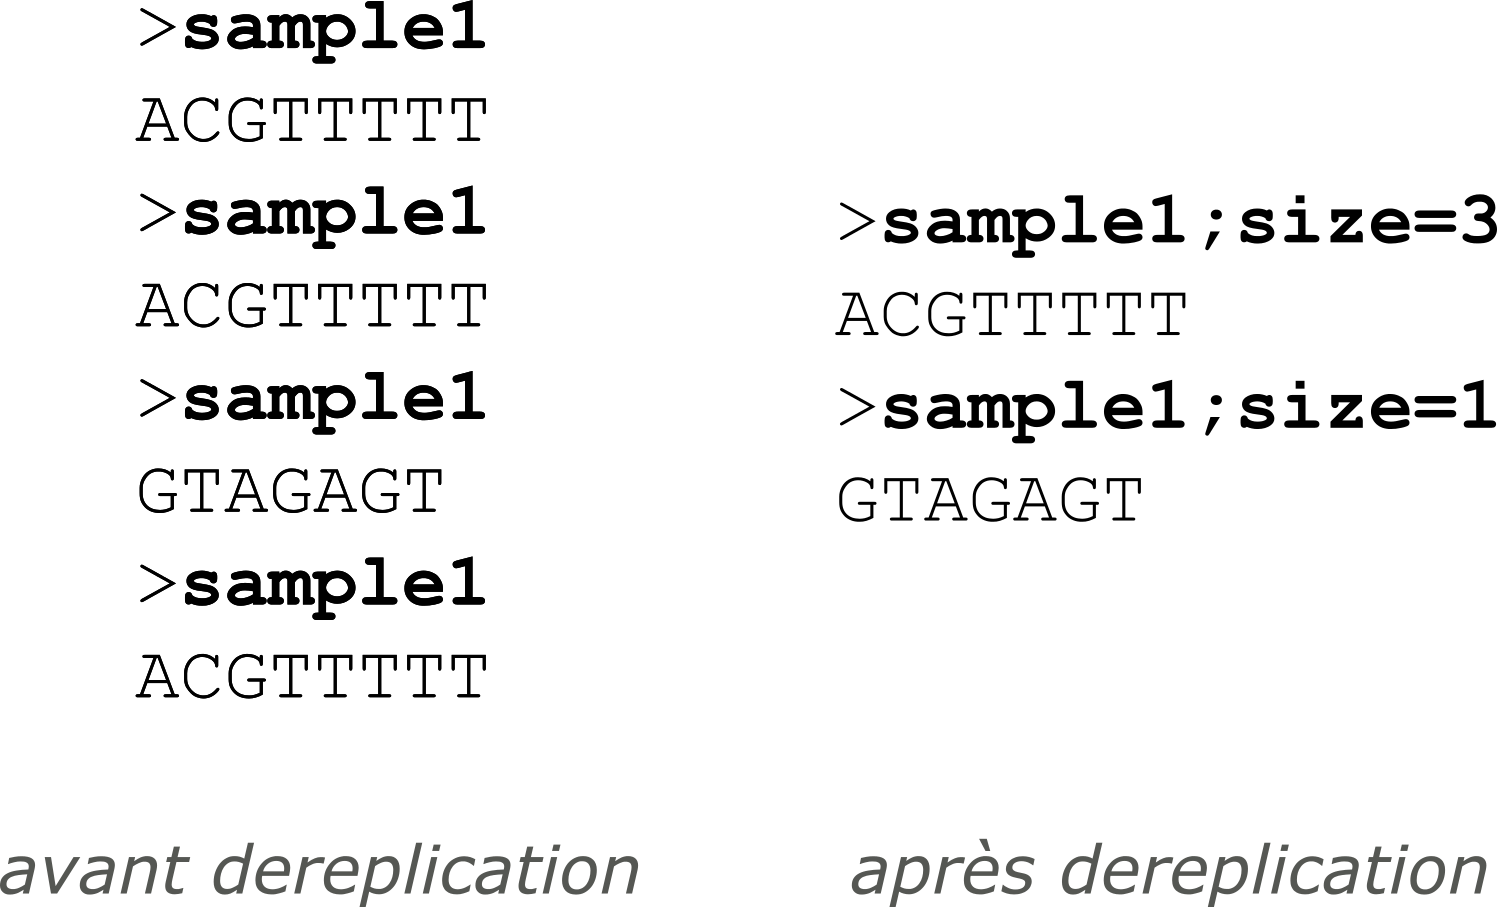
\includegraphics[scale=0.4]{img/dereplication.png}\hfill
\end{center}
\caption{Exemple de déréplication d'un fichier fasta}
\label{dereplication}
\end{figure}

\subsubsection{Assignation taxonomique}
\noindent\emph{2 fasta en entrée,  1 fichier biom  en sortie. }

L’assignement taxonomique consiste à labelliser chaque read à son taxon. Nous avons utilisé la stratégie \textit{close référence} dont le rôle est de comparer chaque read à une base de données avec un seuil de 98 \% de similarité. Cet algorithme est de complexité N. C'est-à-dire que le temps de calcul est directement proportionnel au nombre de reads testé. La base de données \textit{Greengene}\cite{DeSantis2006} version mai 2013  a été utilisée. Il s'agit d'un fichier fasta contenant 1 262 986 séquences et 203 452 OTUs. \\
L'autre stratégie d'assignation \textit{de novo} n'a pas été utilisée. Cette dernière, de complexité $N^{2}$, consiste à comparer les reads entre eux pour former des groupes. Elle s'emploie de préférence pour détecter les bactéries absentes des bases de données. \\
L'assignation taxonomique a été réalisé avec \textbf{vsearch} et sa fonction \textit{--usearch\_global}.

\subsubsection{Analyse de la table des OTUs}
L’analyse de la table des OTUs a été réalisée avec R et le package \textbf{phyloseq}\cite{McMurdie2013}. Les OTUs ont été regroupés par genre bactérien. La normalisation de la table des OTUs s'est faite en pondérant le nombre de reads au total.
Les abondances absolue et relative, la prévalence, la dominance et la courbe de raréfaction ont été mesurées pour chaque échantillon.
Les diversités alpha de type Chao1 et Shannon ont été mesurées sur tous les échantillons. L'évolution de ces indices a été représentée graphiquement dans le temps et par patient.
La diversité bêta a été évaluée grâce une Analyse en Coordonnées Principales utilisant la distance de Bray-Curtis.
Le core microbiota\cite{VanderGast2011} a été calculé. Il est défini comme l’ensemble des taxons retrouvé dans plus de 50 \% des échantillons avec une abondance supérieure à 0,1 \%.
La corrélation entre les genres a été recherchée.
Les catégories Free et Never ont été comparées d’après leurs diversités alpha et bêta.



\section{Résultats}
\subsection{Séquençage et pipeline}
\subsubsection{Données de séquençage}
Après démultiplexage, 188 x 2 fichiers Fastq ont été générés soit deux fichiers par échantillons.
La longueur des reads dans l'ensemble est de 301 paires de bases.
Au total, 115 002 297 reads ont été produits sur deux runs MiSeq (Figure \ref{readcount}). Avec en moyenne 616 900 reads par échantillon. Un minimum de 61 422 reads pour l’échantillon 2154 et un maximum de 1 071 188 pour l’échantillon 3165.


\begin{figure}[ht]
\begin{center}
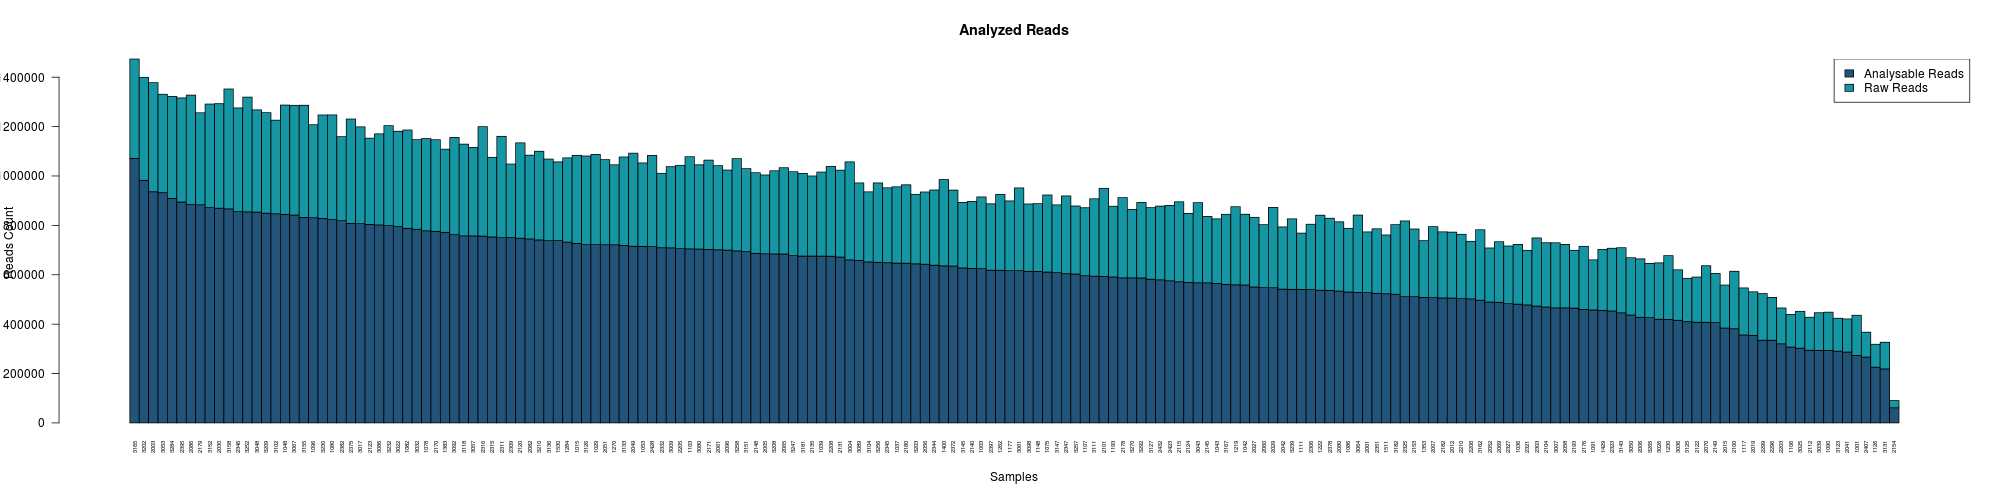
\includegraphics[scale=0.25]{img/pipeline.png}\hfill
\end{center}
\caption{Nombre de reads par échantillon}
\label{readcount}
\end{figure}


\subsubsection{Qualité des reads}
La figure \ref{fastqt} montre la qualité typique d'un fichier fastq produit par le séquenceur. Une baisse de qualité importante est observée à hauteur du 250e nucléotide. Tous les fichiers fastq présentaient le même profil.
À cause de cette baisse de qualité, x \% des reads pairs n'ont pas pu être fusionnés.
L'étape de filtrage a permis de ramener la qualité médiane au-dessus de 20 (Figure \ref{fastqt_after}).
Au total, seulement 49.24 \% des reads ont été conservés pour l'analyse (Figure \ref{readcount}) avec des bornes allant de 37,30 \% à 61,13 \%.



\begin{figure}[ht]
\begin{center}
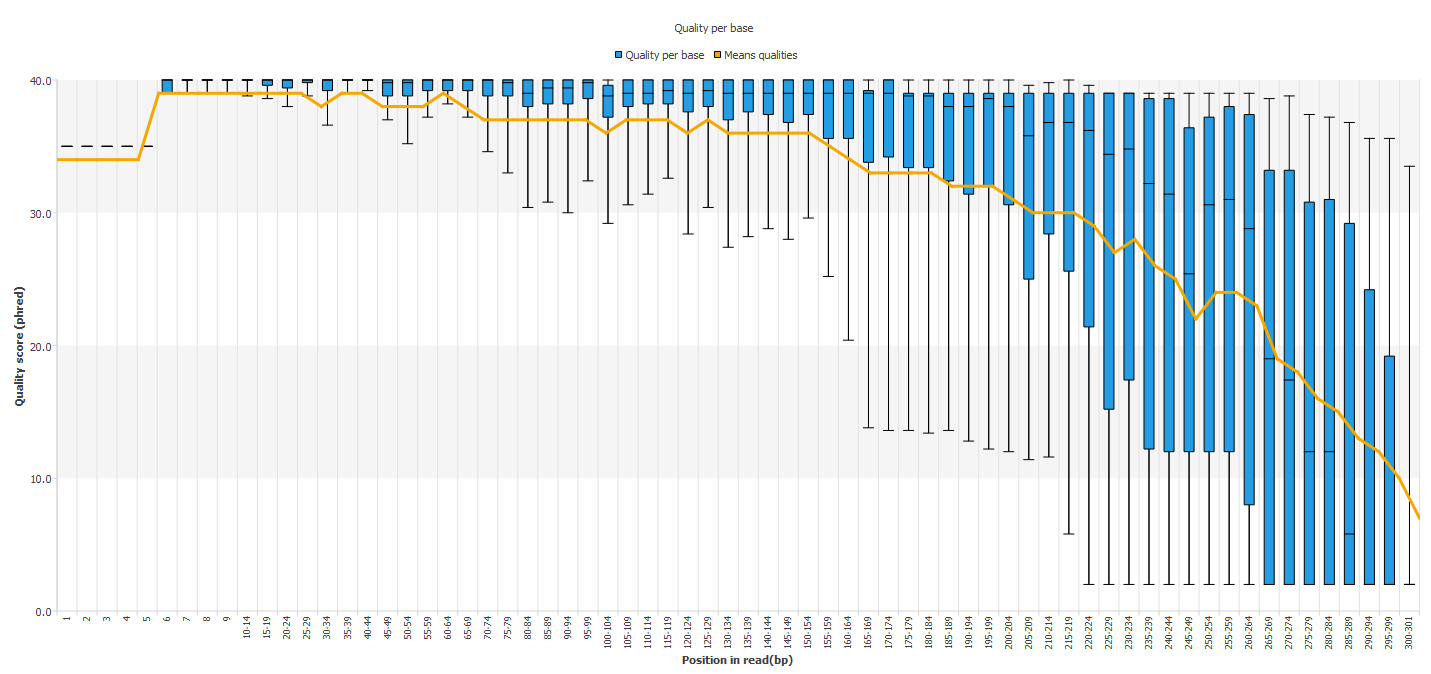
\includegraphics[scale=0.45]{img/1003_forward.png}\hfill
\end{center}
\caption{Qualité par nucléotide des reads forward de l'échantillon 1003. \textbf{Axe X}: la position sur le read. \textbf{Axe Y}: La distribution des qualités}
\label{fastqt}
\end{figure}


\begin{figure}[h]
\begin{center}
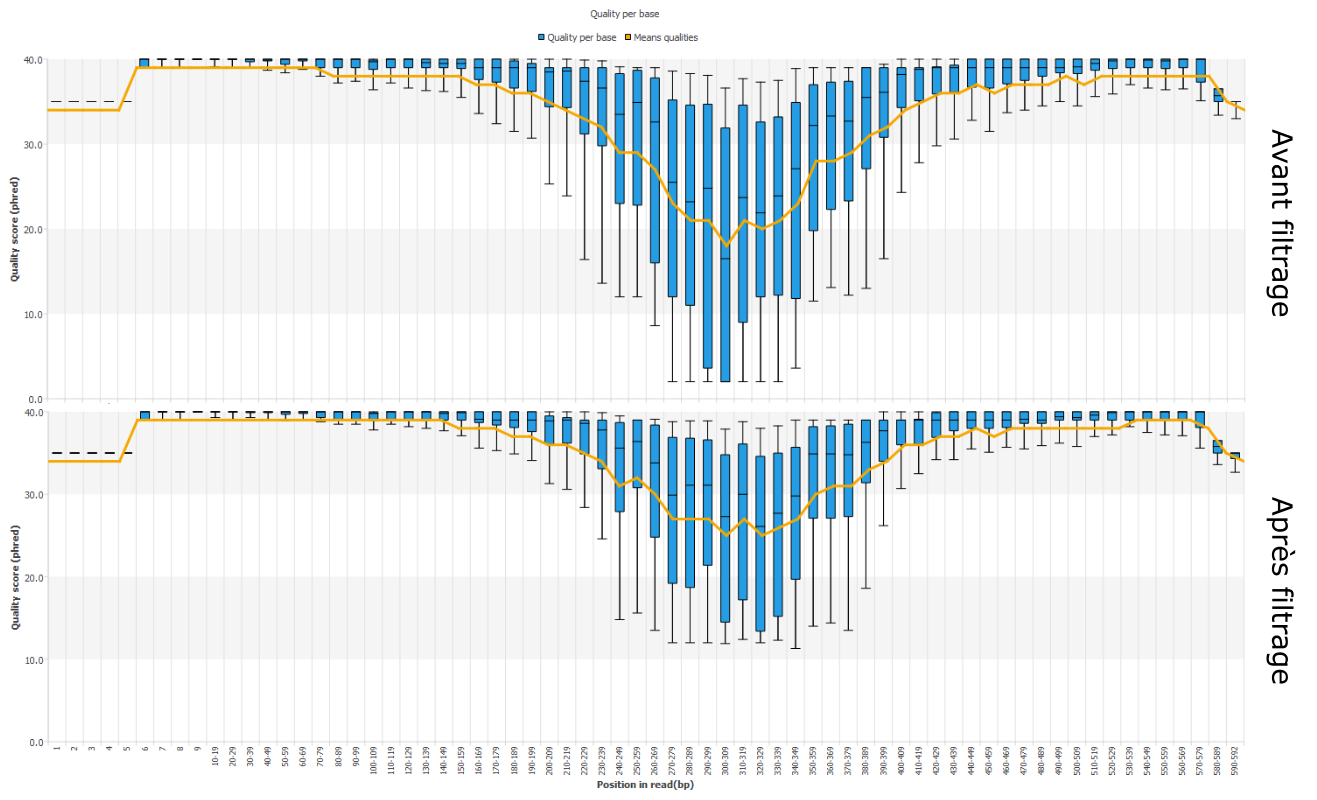
\includegraphics[scale=0.45]{img/duo_merging.png}\hfill
\end{center}
\caption{Qualité par nucléotide des reads fusionnés pour l'échantillon 1003}
\label{fastqt_after}
\end{figure}


\subsubsection{Assignation taxonomique}
99.88 \% (4615960) des reads analysables ont reçu une assignation taxonomique soit 10517 OTUs détectés \footnote{Pour chaque espèce, il y a plusieurs OTUs définis dans \textit{Greengene}} correspondant à 54 genres bactériens (Figure \ref{readgenus}).
Le temps de calcul a été de 1 h 29 et a nécessité 40 cœurs et 20 gigaoctets de mémoire contre 21h de calcul sans l’optimisation par déréplication.


\begin{figure}[h]
\begin{center}
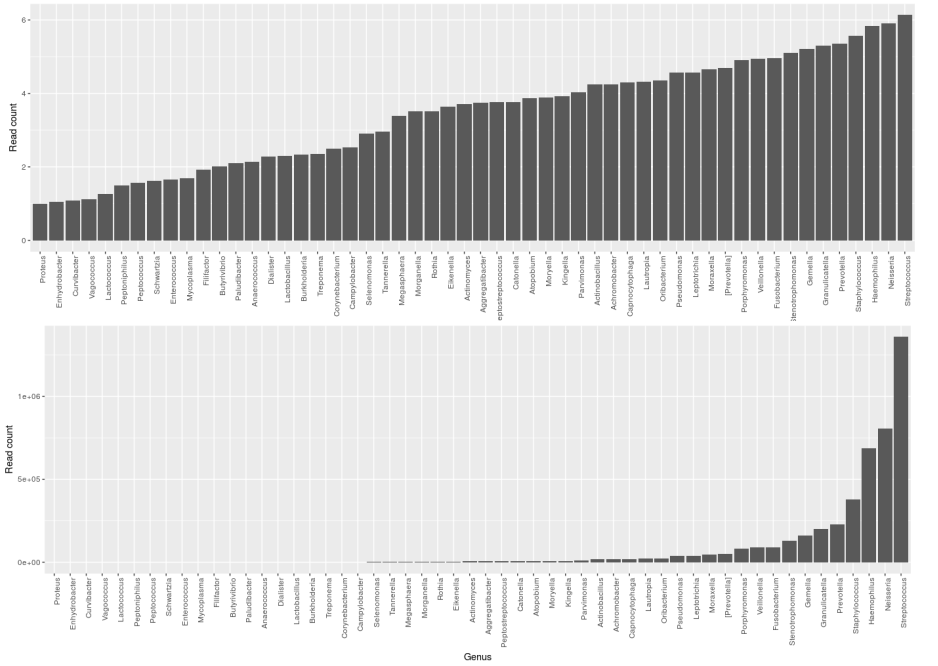
\includegraphics[scale=0.5]{img/read_count_genus_all.png}\hfill
\end{center}
\caption{Nombre de reads par genre bactérien}
\label{readgenus}
\end{figure}


\subsubsection{Profondeur de séquençage}
La figure \ref{rarefaction} montre les courbes de raréfaction pour les 188 échantillons.
Dans l'ensemble elles s’aplatissent précocement, témoignant d’un bon niveau d'échantillonnage. Les quelques échantillons n'ayant pas attend l'asymptote horizontale ont tout de même été conservés.

\begin{figure}[!h]
\begin{center}
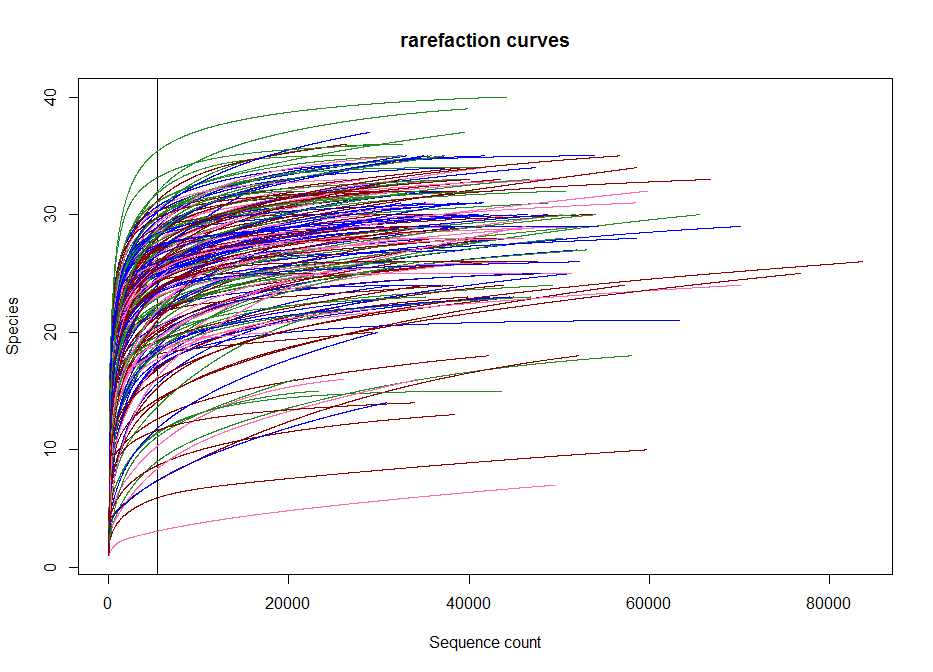
\includegraphics[scale=0.5]{img/rarefaction.png}\hfill
\end{center}
\caption{Courbe de raréfaction pour les 188 échantillons. }
\label{rarefaction}
\end{figure}


\begin{figure}[!ht]
\begin{center}
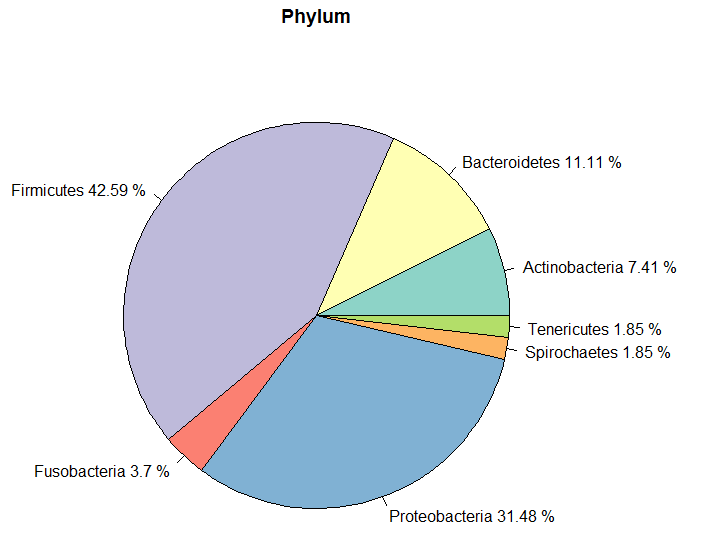
\includegraphics[scale=0.5]{img/phylum.png}\hfill
\end{center}
\caption{Phylums retrouvés dans les 188 échantillons}
\label{phylum}
\end{figure}

\subsection{Résultats descriptifs}
\subsubsection{Composition du microbiote}
Cinquante-quatre genres (Figure \ref{readgenus}) et sept phylums (Figure \ref{phylum}) bactériens sont retrouvés dans l'ensemble des échantillons analysés.
Les deux phyla majoritaires sont \textit{Firmicute} (42.59 \%) et \textit{Proteobacteria} (31.48 \%). Parmi les \textit{Firmicutes} majoritaires, on retrouve \textit{Streptococcus} et \textit{Staphylococcus}. Au sein des \textit{Proteobacteria}, \textit{Neisseria} et \textit{Haemophilus} sont les genres les plus abondants.
Le tableau de la figure \ref{alltable} résume l'ensemble des résultats en y associant la prévalence des genres bactériens parmi les 188 échantillons.
Par exemple \textit{Streptococcus}, \textit{Neisseria}, \textit{Prevotella}, \textit{Granulicatella}, \textit{Gemella}, \textit{Veillonella} et \textit{Fusobacterium} sont très prévalents, car présents dans plus de 185 échantillons.
D’autres genres sont dominants. Il s’agit de \textit{Streptococcus}, \textit{Neisseria}, \textit{Haemophilus} et \textit{Staphyloccoccus}. \textit{Stenotrophomonas} et \textit{Achromobacter} sont retrouvées dans 64 et 8 échantillons respectivement. \textit{Pseudomonas} est retrouvé dans 53 échantillons, dont un, au moins avec une abondance de 25.94 \%. \textit{Burkholderia} est retrouvé seulement dans deux échantillons à moins de 1 \%.\\
Le core microbiota est constitué de 14 genres bactériens (Figure \ref{core}). Sa distribution est illustrée dans la figure \ref{violon}.
\textit{Streptococcus} respecte grossièrement une distribution normale variant de la quasi-absence à la dominance avec une moyenne de 30 \% par échantillon. \textit{Neisseria} est le deuxième genre le plus abondant avec une moyenne de 18 \%.
Les abondances de \textit{Staphylococcus} et \textit{Haemophilus} sont faibles dans la plupart des échantillons. Mais pour quelques échantillons, ces genres sont dominants. Les autres genres ont une abondance faible qui varie faiblement. Ils ne sont jamais retrouvés comme dominants.


\begin{figure}
\begin{center}
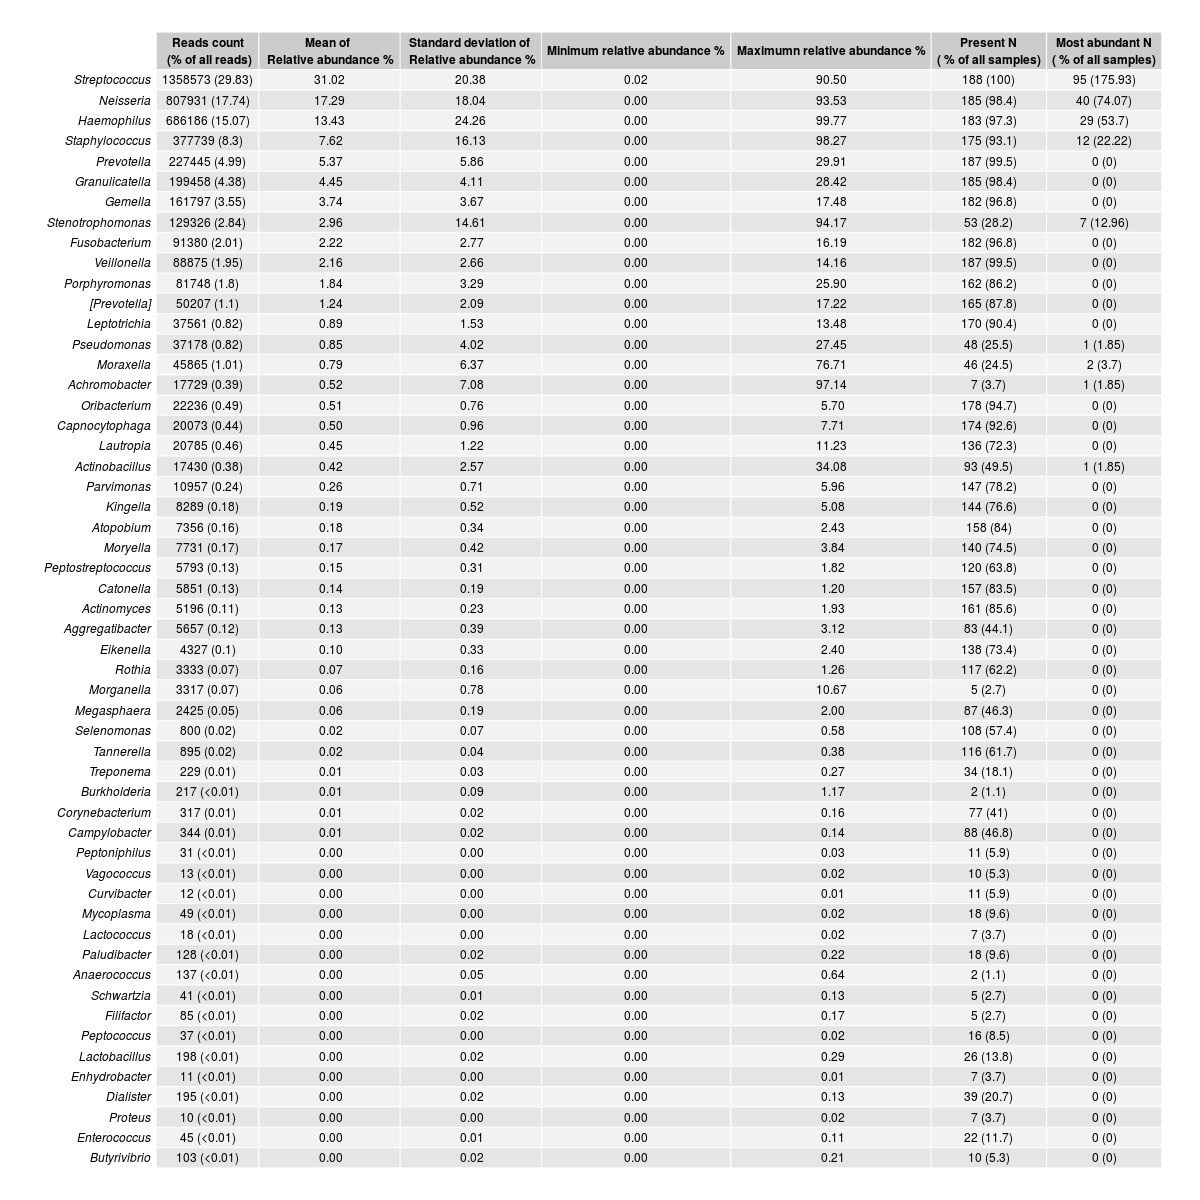
\includegraphics[scale=0.4]{img/alld.png}\hfill
\end{center}
\caption{Résumé détaillé de l'assignation taxonomique des reads. \textbf{Legende:} Nombre de reads - Moyenne des abondances relatives - écart-type des abondances relatives - plus petite abondance relative - plus grande abondance relative - Nombre d'échantillon où le genre est présent - Nombre d'échantillon où le genre est dominant}
\label{alltable}
\end{figure}


\begin{figure}[t]
\begin{center}
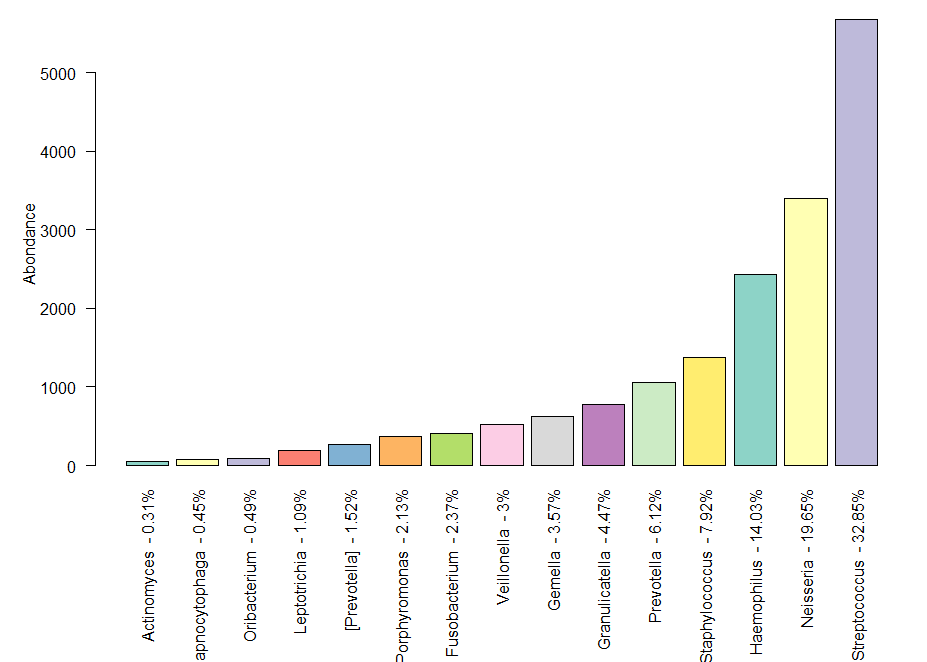
\includegraphics[scale=0.5]{img/core.png}\hfill
\end{center}
\caption{Distribution du core microbiota dans l'ensemble des échantillons}
\label{core}
\end{figure}



\begin{figure}[t]
\begin{center}
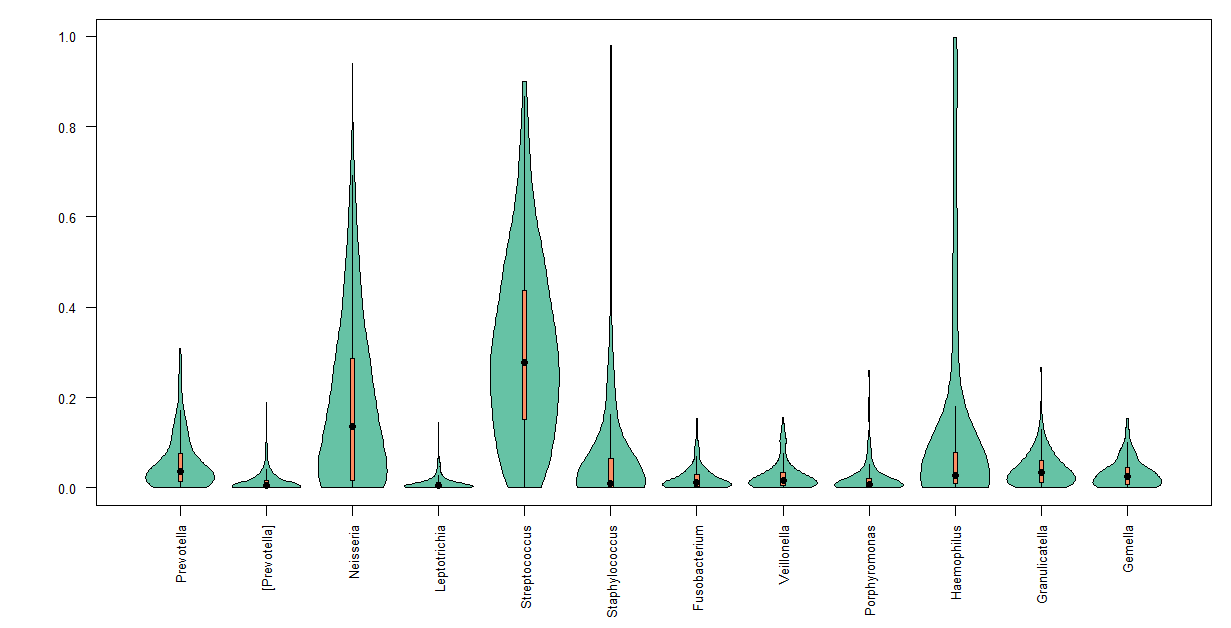
\includegraphics[scale=0.5]{img/variability.png}\hfill
\end{center}
\caption{Variation du core microbiota dans l'ensemble des échantillons}
\label{violon}
\end{figure}

\subsubsection{Évolution de l'alpha diversité}
Les figures \ref{alphaObs},\ref{alphaChao1} et \ref{alphaShannon} en annexe, montrent l’évolution des diversités alpha par patient au cours du temps en utilisant les indices Chao1, Observed et Shannon. \\
La richesse (Observed , Chao1) par patient varie de 10 à 40 genres bactériens. La richesse du patient 256 est faible. Celle du patient 26 élevée.
Certains patients ont des richesses stables au court du temps. Les patients 25, 26 et 74 conservent leurs richesses sur plus de 5 prélèvements successifs. Les patients 20 et 69 présentent une stabilité globale entrecoupée par des pertes de biodiversité. La richesse du patient 8 diminue progressivement. Les patients 23, 232 et 248 ont des fluctuations plus chaotiques.
L'indice de Shannon montre que pour un richesse constante dans le temps, l'équitabilité est différente. Par exemple, la richesse du patient 223 est stable sur la figure, \ref{alphaObs} mais son indice de shannon varie sur la figure \ref{alphaShannon} témoignant d'une distribution différente de ses bactéries. Seul le patient 26 semble conserver à la fois une richesse et une équitabilité stables au court du temps.

\subsubsection{Évolution des abondances}
Les figures \ref{plotabundancegenre}, \ref{plotabundancephylum} et \ref{plotabundancecurve} montrent l’évolution des abondances au cours du temps pour chaque patient. Ces graphiques nous permettent d’interpréter plus finement les graphiques d’alpha diversité précédents.
Par exemple, la diminution de richesse du patient 8 est liée à la présence de \textit{Stenotrophomonas} sur les 4 échantillons.
La perte de diversité du 3e prélèvement du patient 223 est causée par l'apparition de \textit{Neisseria} qui devient dominant.
Le patient 3 montre une diminution progressive \textit{d’Haemophilus} parallèlement à une augmentation de \textit{Streptococcus}. \\
Le patient 256 présente une dominance à \textit{Stenotrophomonas} sur l'ensemble de ses échantillons. \textit{Achromobacter} est dominant dans le premier échantillon du patient 211.
D’autres montrent un phénomène de résilience. Par exemple, le patient 223 récupère un microbiote identique après une colonisation quasi omnisciente à \textit{Haemophilus}. \\
Dans l’ensemble, il existe deux types de population bactérienne: une population de bactéries constantes et minoritaires (\textit{Fusobacterium}, \textit{Granulicatella}, \textit{Gemella}, \textit{Veillonella}, \textit{Parvimonas}, \textit{Leptotrichia},\textit{Oribacterium}, \textit{Capnoctophaga},\textit{Catonella}); une autre population de bactéries très fluctuantes dans le temps jouant alternativement le rôle de genre dominant ou au contraire de genre absent. (\textit{Haemophilus}, \textit{Streptococcus}, \textit{Neisseria} et \textit{Prevotella}).
La figure \ref{evolution43} zoome sur le patient 43 pour montrer ces deux populations. La figure du patient \ref{evolution54} est mise également à titre exemple, car elle montre l’apparition de \textit{P. aeruginosa}. \\

\begin{figure}
\begin{center}
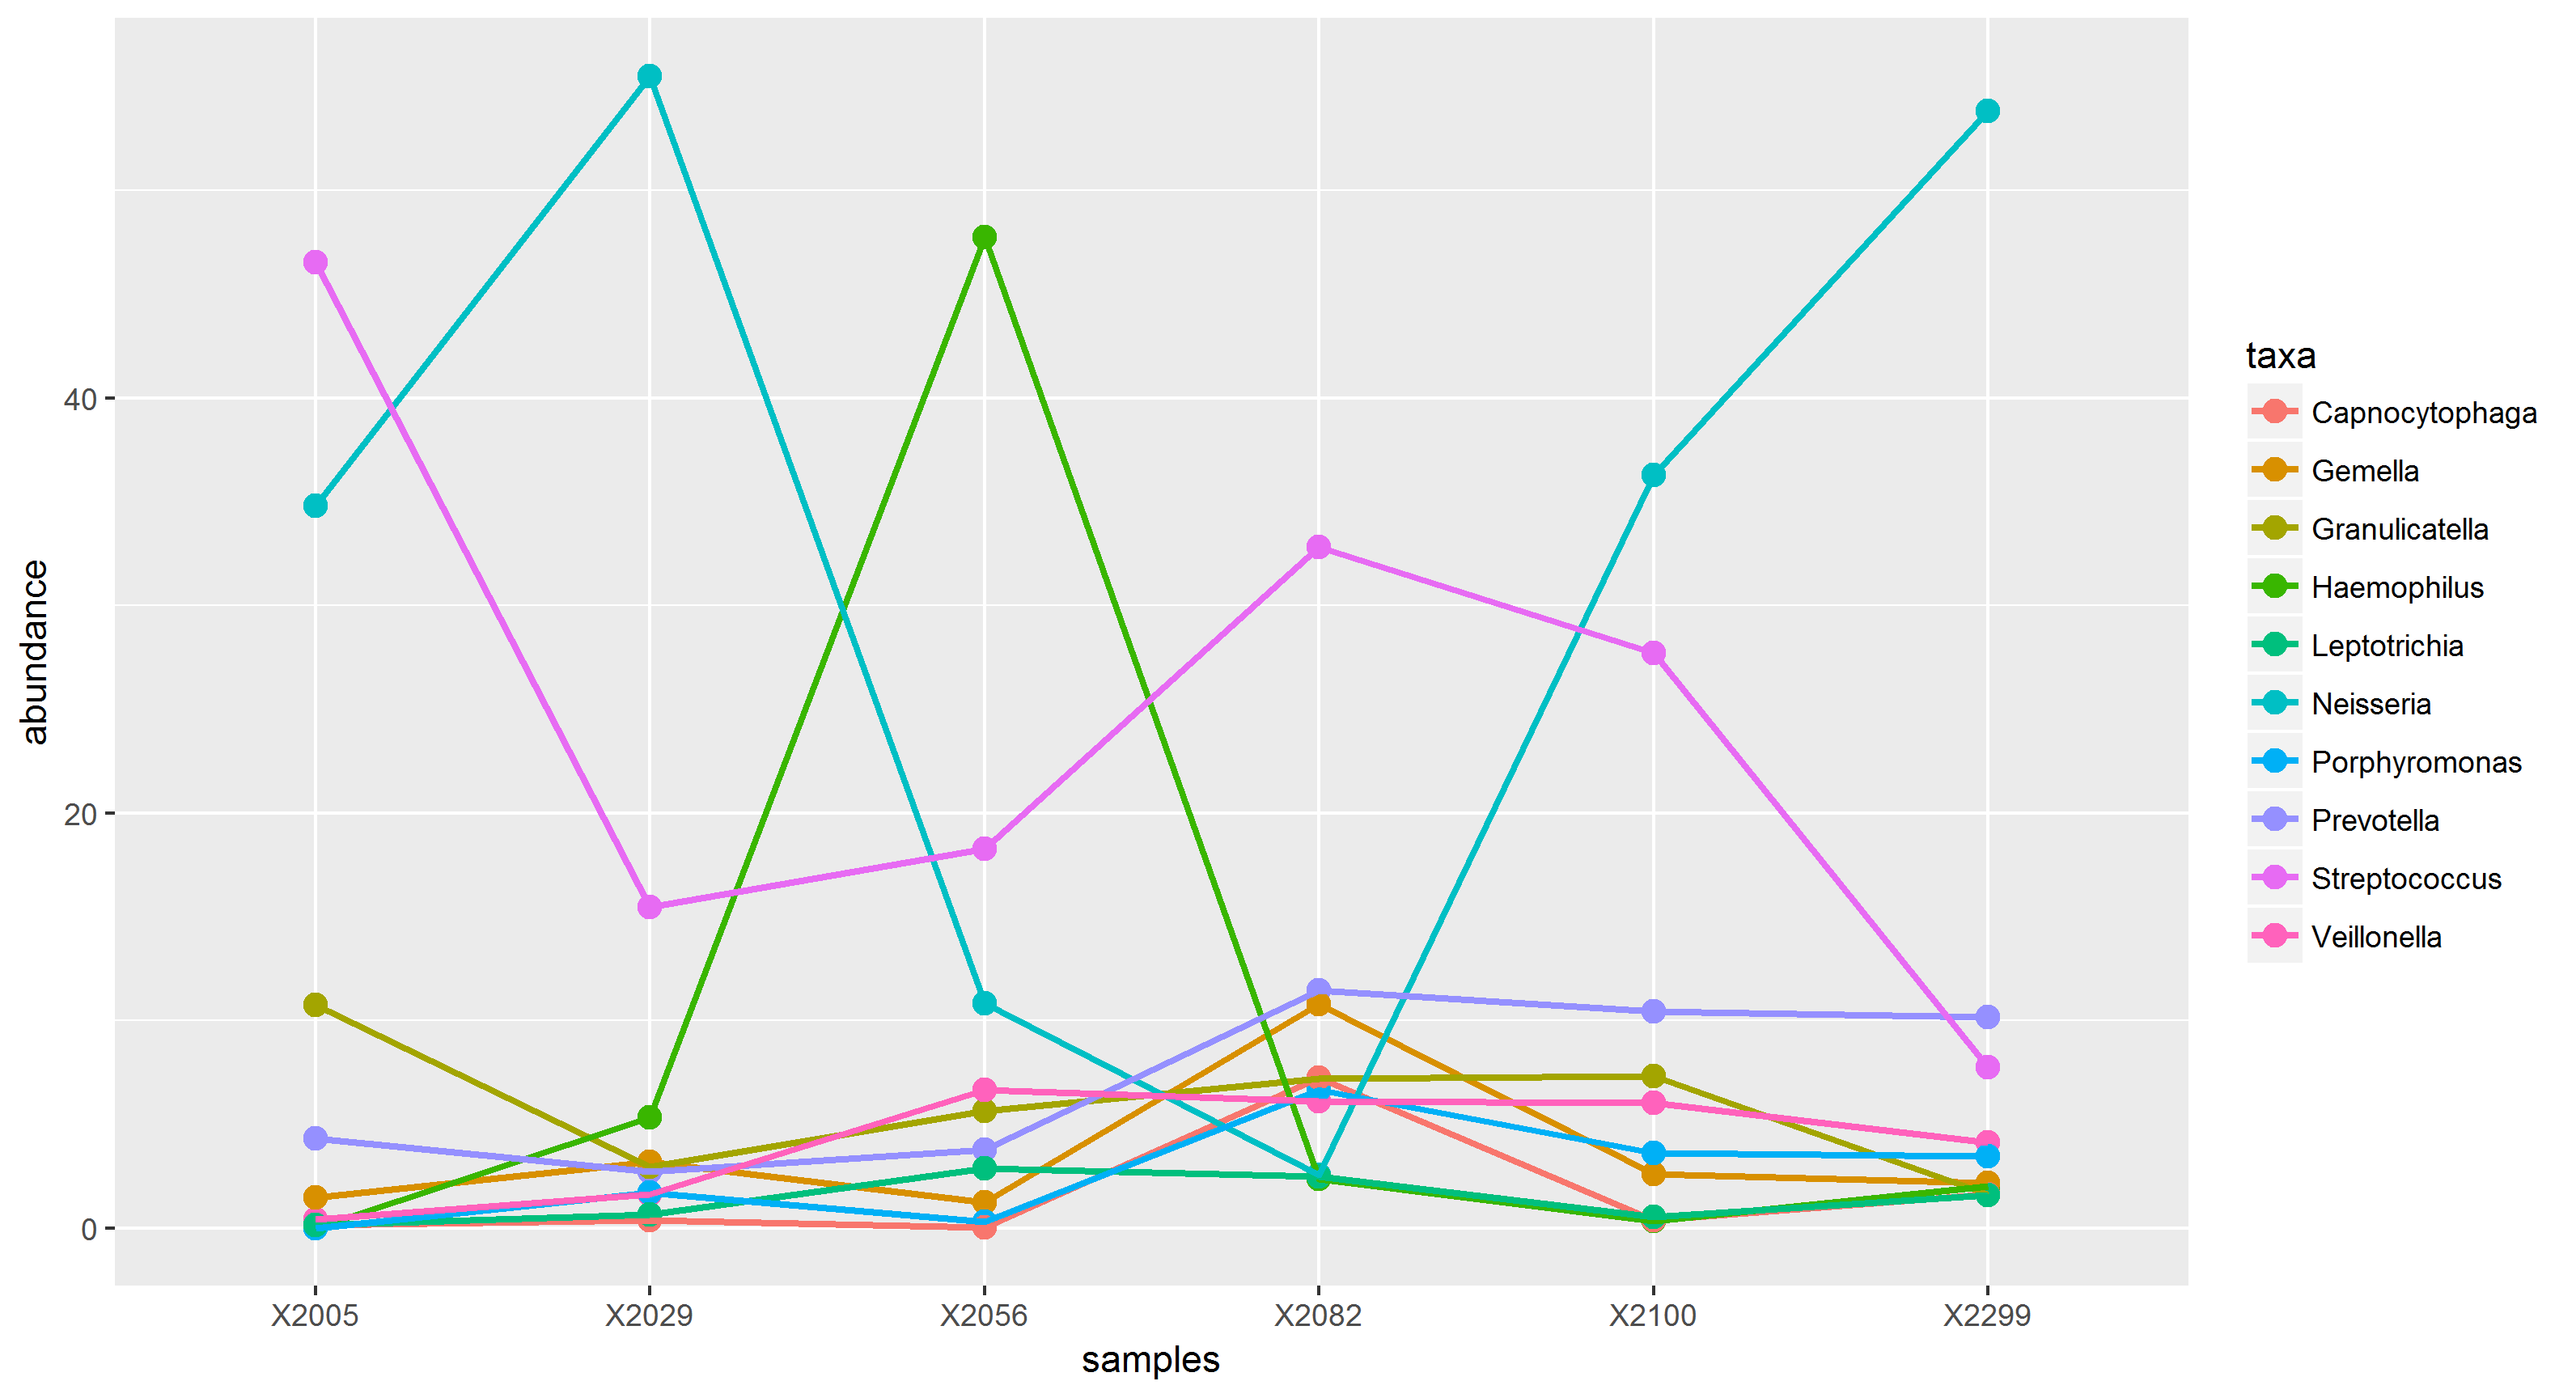
\includegraphics[scale=0.60]{img/curve_043.png}\hfill
\end{center}
\caption{Évolution des abondances pour le patient 43. Notez la population stable et la population fluctuante}.
\label{evolution43}
\end{figure}

\begin{figure}
\begin{center}
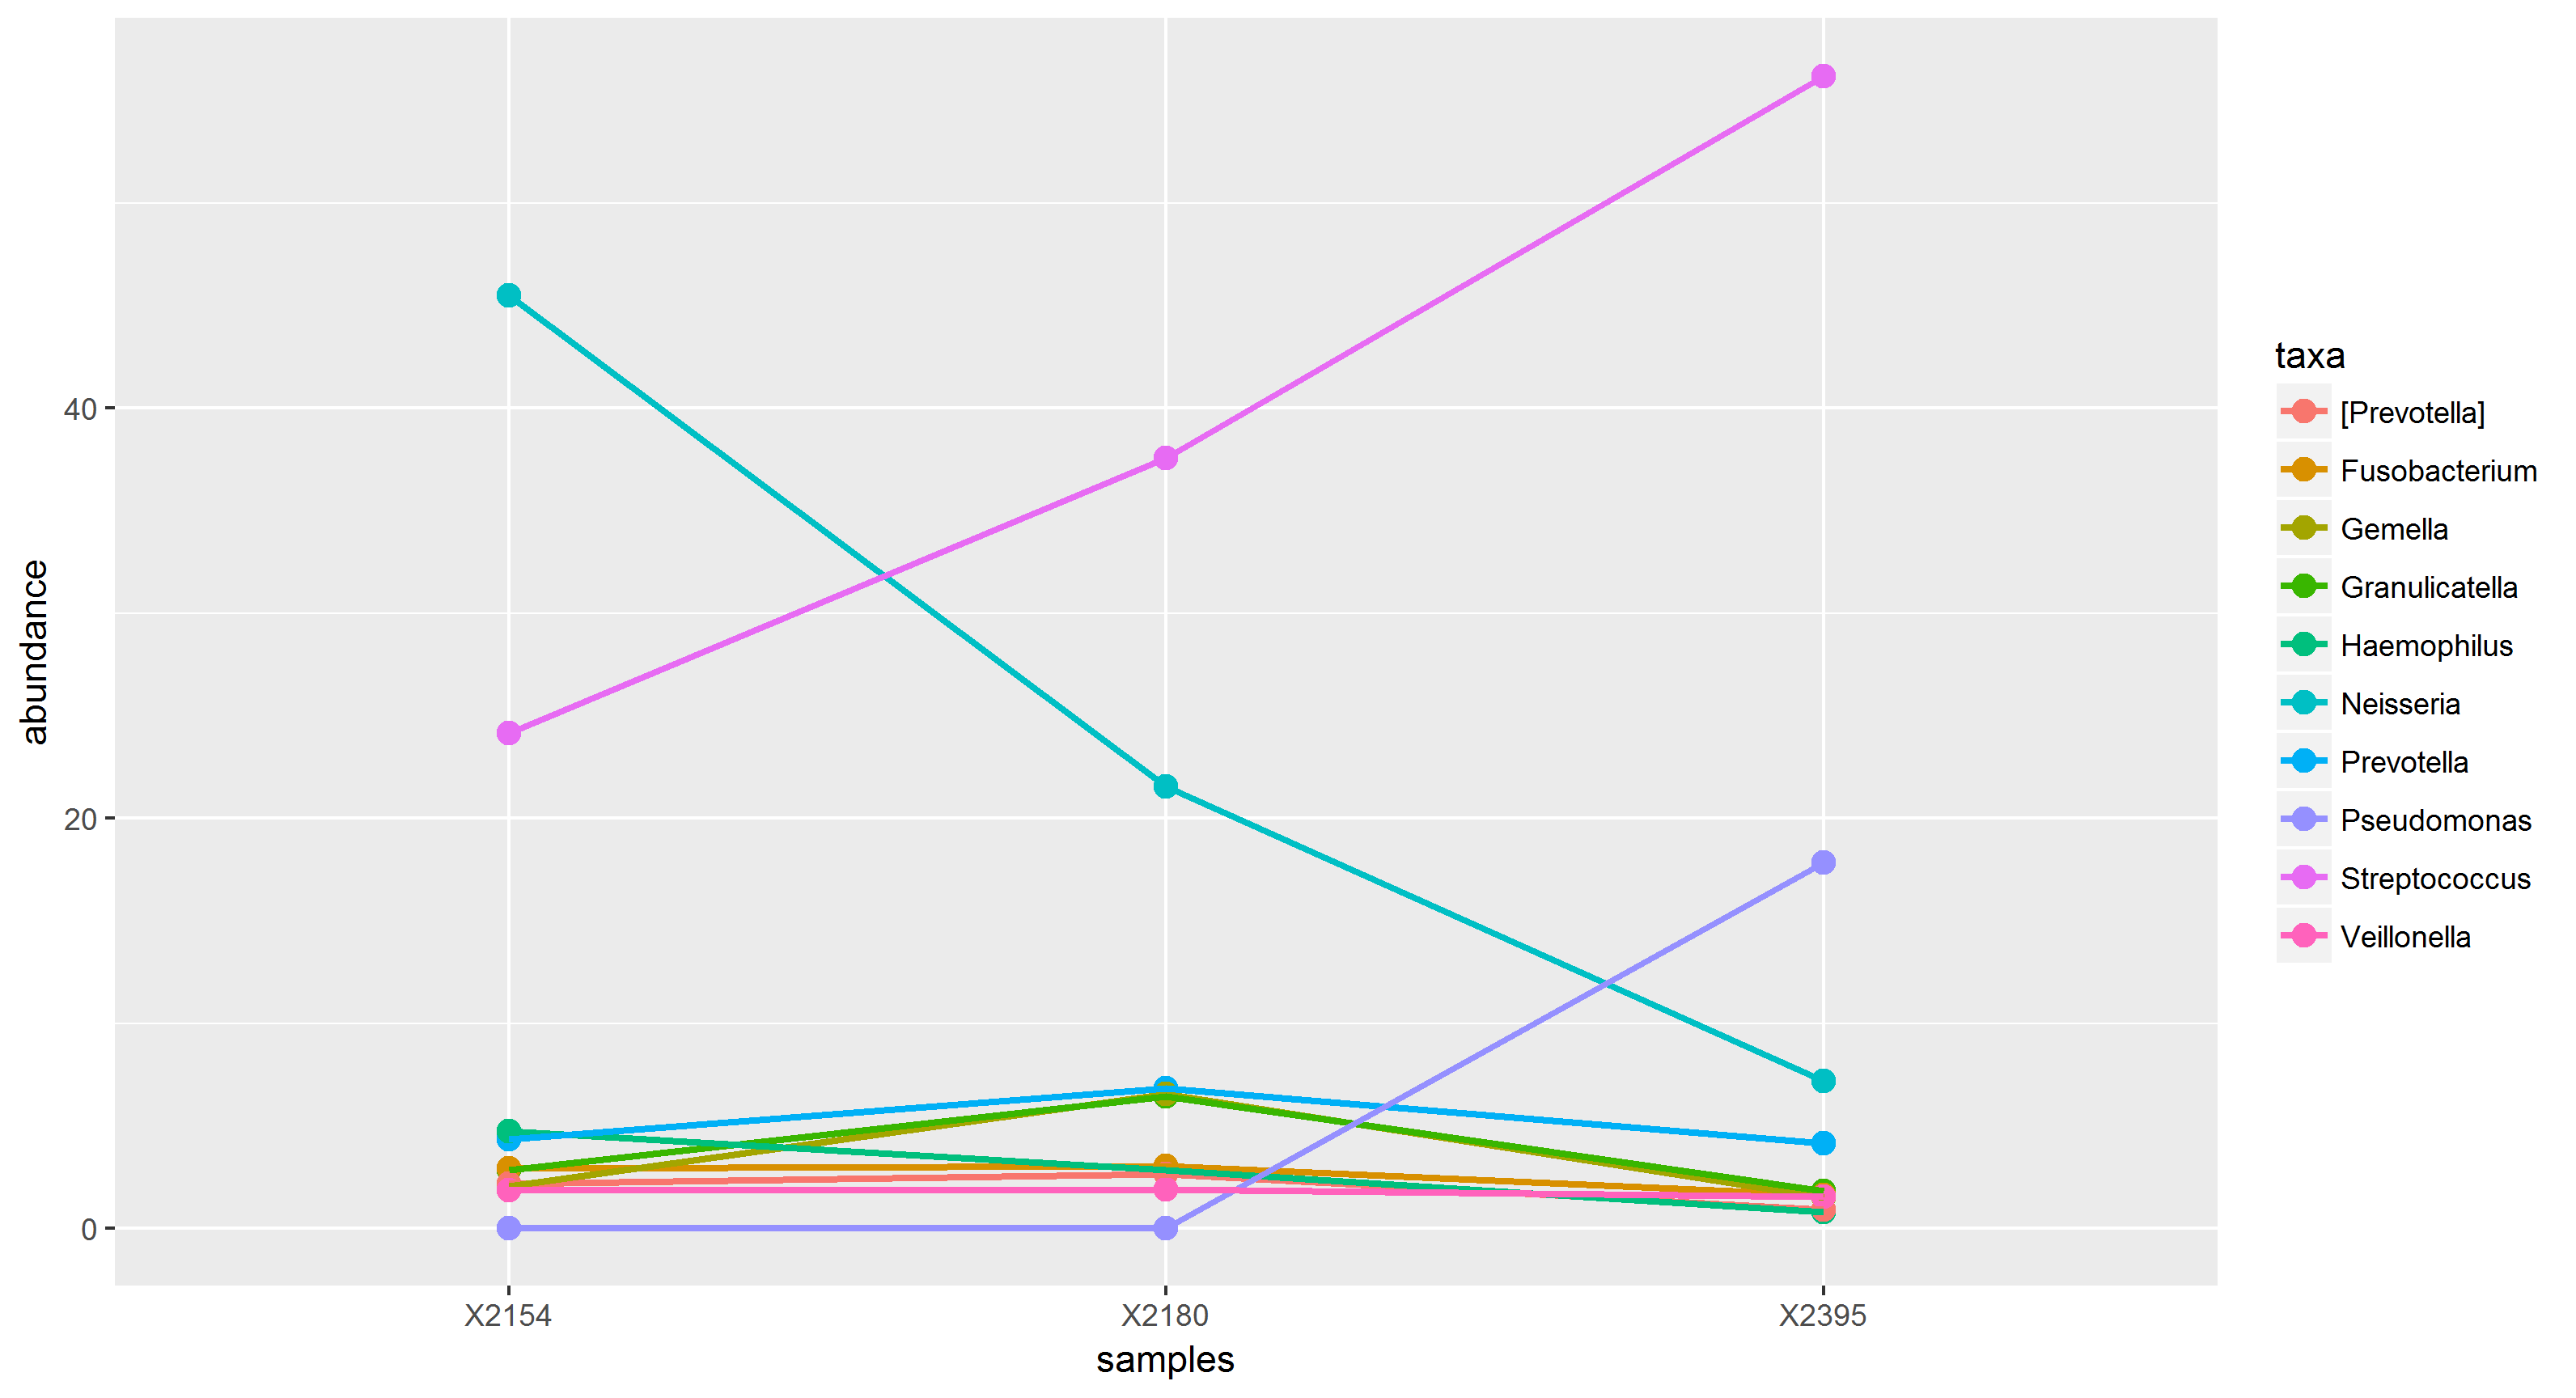
\includegraphics[scale=0.60]{img/curve_054.png}\hfill
\end{center}
\caption{Évolution des abondances pour le patient 54. Notez l'apparition de \textit{Pseudomonas} dans le dernier échantillon}.
\label{evolution54}
\end{figure}

\subsubsection{Bêta Diversité}
La bêta diversité sur l’ensemble des échantillons a été réalisée par une méthode d’ordination de type PCoA en utilisant les distances de Bray-Curtis (Figure \ref{ordination},\ref{ordination2} et \ref{pcoa}).
Les deux axes principaux expliquent respectivement 28.5 \% et 17.4 \% de la variabilité.
Certains échantillons d’un même patient sont très proches sur le graphique d’ordination. Par exemple le patient 69 et 003 ont des échantillons dont les points se confondent.
Aucune des analyses tenant compte des paramètres biocliniques colligés pendant l'étude MUCOBIOME comme l'âge, le sexe, le poids, la prise d'antibiotique et le type de mutation du gène \textit{CFTR} n’a mis en évidence des groupes distincts de microbiote. Le score cytologique n'a pas non plus montré de différence.
La variabilité est expliquée principalement par la dominance des genres \textit{Neisseria}, \textit{Streptococcus} et \textit{Haemophilus} comme le montre la figure \ref{ordination2}.


\begin{figure}
\begin{center}
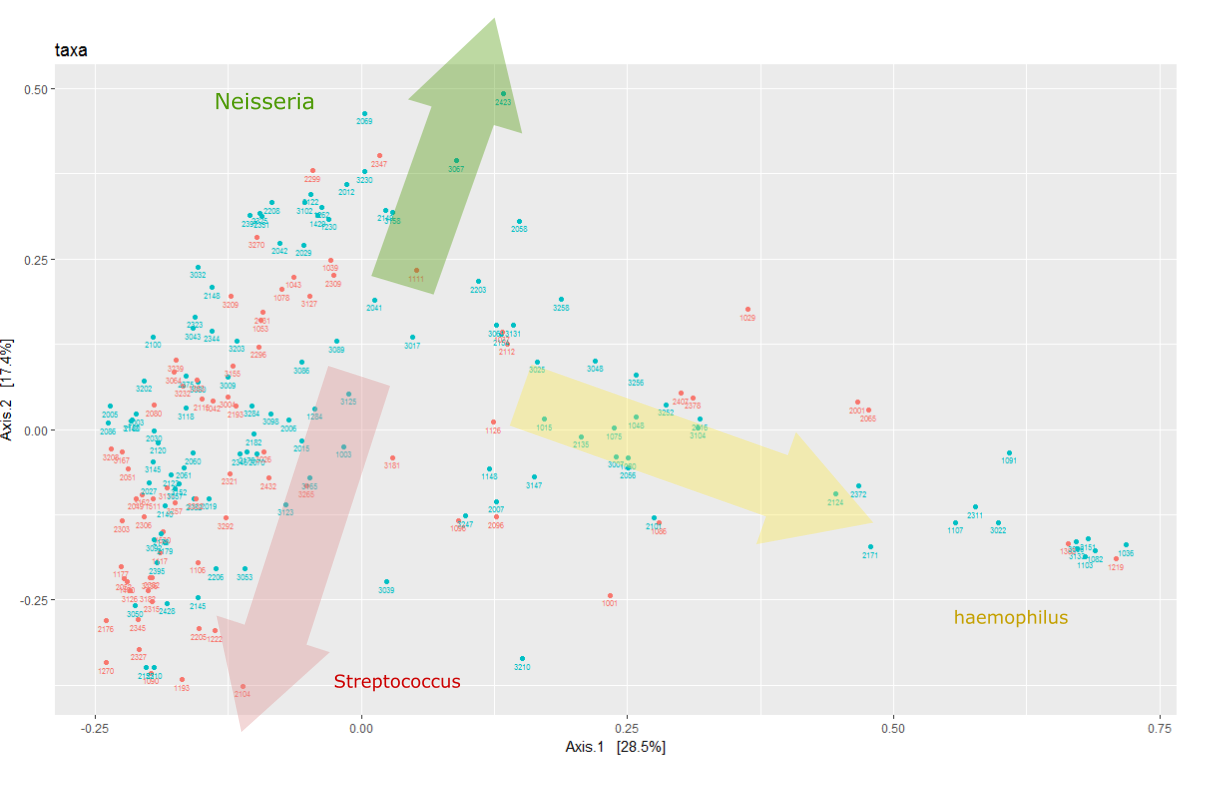
\includegraphics[scale=0.50]{img/Capture.png}\hfill
\end{center}
\caption{Analyse en coordonnées principales sur les 188 échantillons en utilisant les distances de Bray-Curtis. Chaque point est un échantillon labellisé par l'identifiant du patient. La variabilité s'explique principalement par \textit{Haemophilus}, \textit{Streptococcus} et \textit{Neisseria}}
\label{ordination2}
\end{figure}


\begin{figure}
\begin{center}
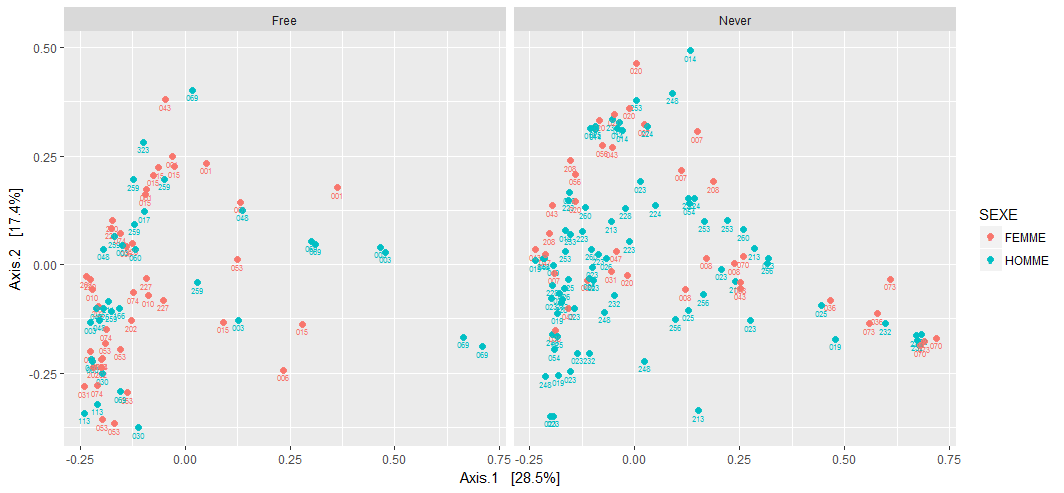
\includegraphics[scale=0.62]{img/oordination_new.png}\hfill
\end{center}
\caption{Analyse en coordonnées principales sur les 188 échantillons en utilisant les distances de Bray-Curtis. A gauche les échantillons Free, à droite les échantillons Never. Le sexe est mis en couleur à titre indicatif.}
\label{ordination}
\end{figure}

\subsubsection{Présence de P. aeruginosa}
Sur les 188 échantillons, 22 étaient positifs à \textit{P.aeruginosa} en culture. L'ADNr 16S de Pseudomonas est détecté dans 48 échantillons. Dans la majorité des cas, l'abondance relative est faible. Sur les 48 échantillons, 39 ont une abondance relative en dessous de 3 \%. L'abondance la plus forte est de 27,4 \% et correspond au "end point" positif en culture du patient 10.
Les tableaux \ref{pyopcr} et \ref{pyoculture} comparent le nombre d'échantillons arborant des reads ADNr 16S de \textit{P.aeruginosa} avec ceux détectés par qPCR (données de l'étude de Héry-Arnaud et al., 2017) et par culture.

  \begin{table}[!h]
      \centering
      \begin{tabular}{r|c|c}
           & PCR négative  & PCR positive \\
           \hline
           16S absent & 141 & 31 \\
           16S présent & 1 & 15   \\

      \end{tabular}
      \caption{Concordance entre la présence d'ADNr 16S de Pseudomonas et sa détection en qPCR oprL}
      \label{pyopcr}
  \end{table}

  \begin{table}[!h]
      \centering
      \begin{tabular}{r|c|c}
           & Culture négative  & Culture positive \\
           \hline
           16S absent & 163 & 9 \\
           16S present & 3 & 13   \\
      \end{tabular}
      \caption{Concordance entre la présence d'ADNr 16S de Pseudomonas et sa détection en culture}
      \label{pyoculture}
  \end{table}


\subsection{Résultats analytiques}
\subsubsection{Corrélation entre les genres bactériens}
La figure \ref{correlation} montre les corrélations linéaires réalisées entre les genres du core microbiota. La corrélation la plus forte est entre \textit{Prevotella} et \textit{Veillonella} avec un coefficient de Pearson à 0.60.  \textit{Streptococcus} et \textit{Haemophilus} évoluent dans le sens inverse avec un coefficient à -0.41.


\begin{figure}
\begin{center}
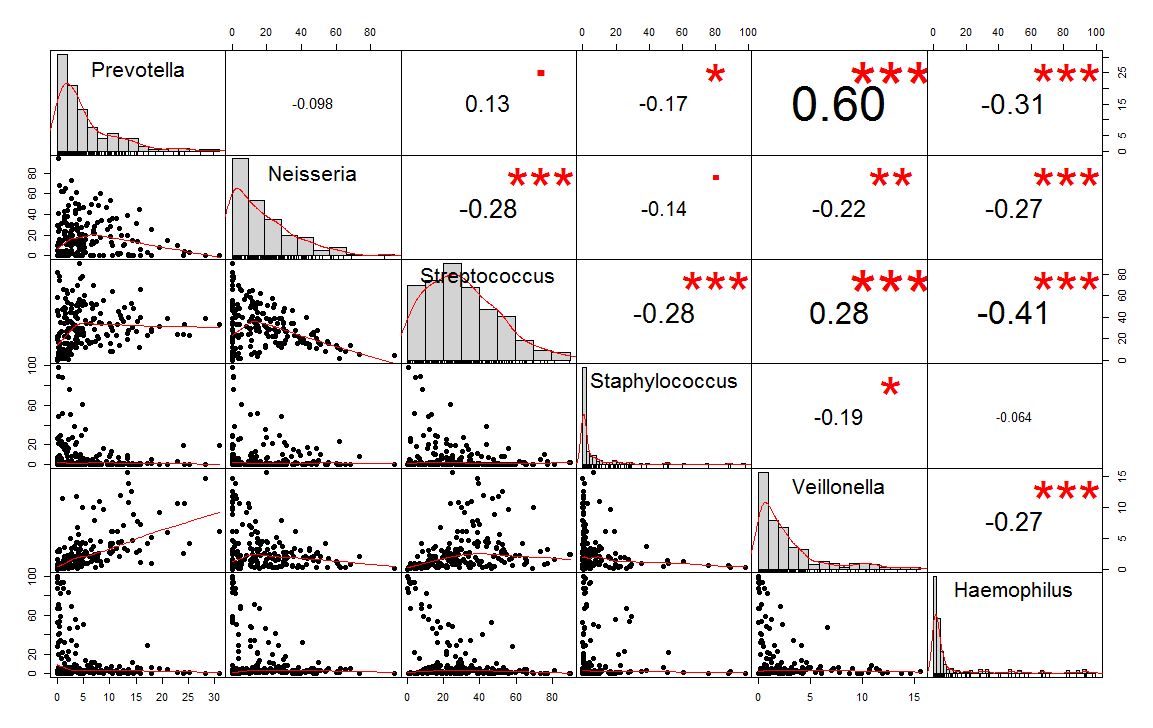
\includegraphics[scale=0.50]{img/small_correlation.png}\hfill
\end{center}
\caption{Corrélation des abondances entre les genres du core microbiota}
\label{correlation}
\end{figure}

\subsubsection{Comparaison entre échantillons Free et Never}
La figure \ref{compare} compare les indices de Shannon entre les échantillons Free et Never. Le T-test / ANOVA n'a pas montré de différence significative (p-value > 0.05). \\
La figure  \ref{pcoa} est une analyse multivariée discriminant les groupes Free et Never. Les échantillons Never ont plus de différences entre eux que les échantillons Free qui semblent converger.  Les deux groupes sont significativement différents p-value < 0.001.

\begin{figure}
\begin{center}
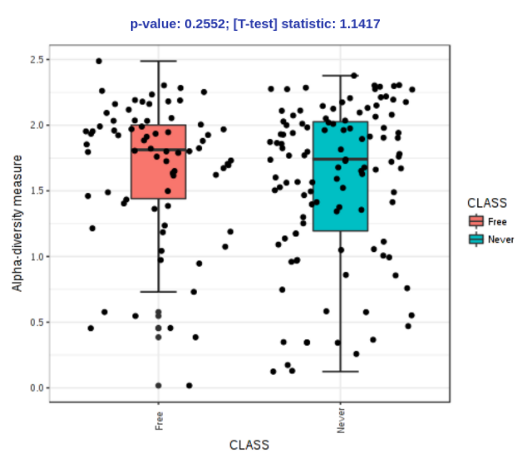
\includegraphics[scale=0.70]{img/compare.png}\hfill
\end{center}
\caption{Comparaison des diversités de Shannon entre les échantillons Free et Never}
\label{compare}
\end{figure}


\begin{figure}[t]
\begin{center}
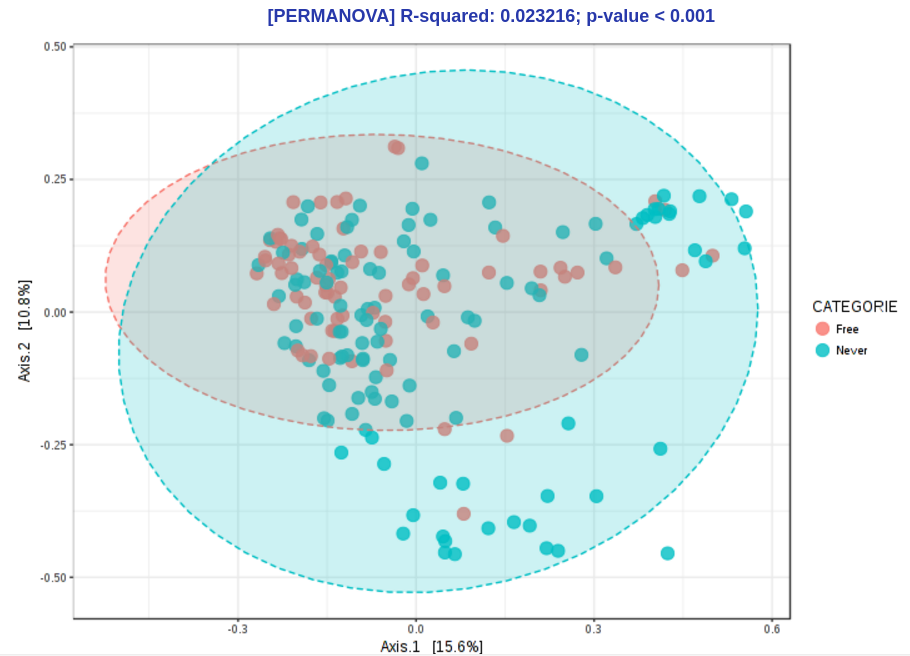
\includegraphics[scale=0.50]{img/pcoa.png}\hfill
\end{center}
\caption{Permanova entre les échantillons Free et Never sur une PCoA en utilisant la distance de Bray-Curtis}
\label{pcoa}
\end{figure}

\newpage
\section{Discussion}
\subsection{Production des données}
\subsubsection{Séquençage}
La version 3 du kit MiSeq Reagent Kit produit des reads plus longs (300 pb) que dans la version précédente (250 pb) afin d'augmenter la précision de l'assignation taxonomique (Figure \ref{rnasens}). En contrepartie la qualité du séquençage est médiocre aux extrémités avec des scores qui chutent en dessous de 20. À cause de cela, seulement 43 \% de reads sont exploitables.
C'est un problème connu lié à la chimie du kit que Illumina n'a pas corrigé à ce jour. La profondeur de séquençage reste toutefois suffisante comme l'attestent les courbes de raréfaction. En utilisant d'autres amorces ciblant des régions de l'ADNr 16S différentes, nous pourrions augmenter la taille du chevauchement pour gagner en profondeur, mais en diminuant la longueur des reads. \\
Les séquenceurs de 3e générations comme le Mini Ion (Oxford Nanopore) ou le PacBio (Pacific Bioscience) apporteraient un avantage certain. Ces derniers sont capables de produire des reads très longs (10 000 pb en moyenne) et pourraient facilement séquencer l'intégralité de l'ADNr 16S. De plus, contrairement à Illumina, les fragments d'ADN sont directement lus (Technologie SMS: Single Molecule Sequencing) évitant ainsi tout biais d'amplification pouvant surévaluer les abondances.
La qualité des reads de ces séquenceurs de 3e génération est en revanche de mauvaise qualité. Malgré cela, deux études\cite{Wagner2016,Benitez-Paez2016} ont déjà montré que leurs résolutions taxonomiques atteignent facilement celui de l’espèce.

\begin{figure}
\begin{center}
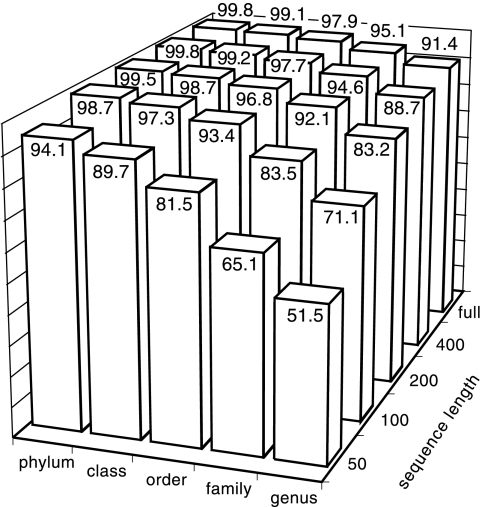
\includegraphics[scale=3]{img/zam.jpg}\hfill
\end{center}
\caption{Sensibilité de détection de la stratégie 16S en fonction de la longueur des reads. (Wang et al. Naïve Bayesian Classifier for Rapid Assignment of rRNA Sequences into the New Bacterial Taxonomy) }
\label{rnasens}
\end{figure}

\subsubsection{Pipeline}
La stratégie close-reference utilisée dans le pipeline mucobiome a permis d'assigner jusqu'au niveau du genre, plus de 99 \% des reads analysés. La base de données \textit{Greengene} est donc assez exhaustive pour analyser le microbiote respiratoire, car tous les genres sont connus.
En revanche, la résolution taxonomique n'atteint pas le rang de l'espèce. Il a en effet déjà été montré que les régions hypervariables prises isolément ne sont pas assez discriminantes \cite{Yang2016}. Deux espèces peuvent par exemple varier d'un seul nucléotide dans une région hypervariable.
D'autre part, l'assignation taxonomique dépend d'une similarité fixée arbitrairement à 97 \%. D'autres algorithmes permettent de s'affranchir de ce seuil. Il s'agit par exemple de la clusterisation par calcul d'entropie maxium \textit{Maximum entropy clusterisation} \cite{Bobadilla2015}.


\begin{figure}
\begin{center}
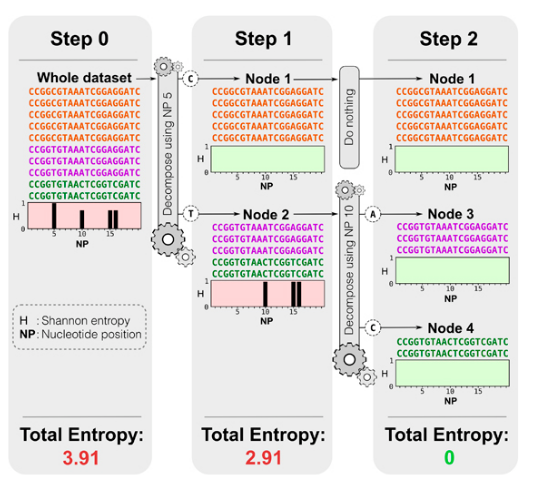
\includegraphics[scale=0.7]{img/entropy.png}\hfill
\end{center}
\caption{Principe de la décomposition par entropie minimum\cite{Bobadilla2015}. Étape 1: les reads sont alignés. L'entropie H est calculée pour chaque position nucléotidique. Étape 2: La position ayant la plus forte entropie est utilisée pour discriminer deux groupes. Étape 3 : Le processus est répété jusqu'à atteindre une entropie totale de 0 }
\label{entropy}
\end{figure}
\subsubsection{Méthodes d'analyse}
Parmi les analyses de bêta diversité, seule l'analyse en coordonnées principales a été présentée en utilisant la distance de Bray-Curtis.
Nous avons également réalisé d'autres ordinations (données non montrées) qui n'ont pas été concluantes. Par exemple, en changeant le type de distance ou en utilisant un positionnement multidimensionnel (MDS) au lieu de la PCoA. \\
Par ailleurs, la proximité phylogénétique des bactéries n'a pas été prise en compte. Un microbiote contenant trois bactéries proches n'est pas la même chose qu'un microbiote contenant trois bactéries très éloignées.
La distance UniFrac\cite{Lozupone2005} pourrait alors remplacer la distance de Bray-Curtis en prenant en considération la phylogénie des bactéries.


%[https://www.ncbi.nlm.nih.gov/pmc/articles/PMC5382435/]
% to gut microbiota, the ‘core' airway microbiota in healthy lungs is predominantly %comprised of the phyla Bacteroidetes, Firmicutes and Proteobacteria, followed by %lesser proportions of Actinobacteria.28, 32, 33

\subsection{Analyse des données}
\subsubsection{Principaux phyla bactériens}
Par rapport aux données chez les sujets sains \cite{Marsland2014}, nos résultats chez les patients mucoviscidosiques montrent une augmentation des \textit{Proteobacteria} (31.48 \%) aux dépens des \textit{Bacteroidetes} (11.11 \%). Et dans une moindre mesure, une augmentation des \textit{Actinobacteria} (7.41 \%). Ces résultats sont en accord avec ceux présentés dans la méta-analyse de \textit{Nature} retrouvant ces proportions dans la mucoviscidose, l'asthme et la BPCO. Cet excès s’explique principalement par la dominance d’\textit{Haemophilus} et de \textit{Neisseria}.  
Par ailleurs, une large proportion d’anaérobies est retrouvée, avec notamment   \textit{Prevotella} et \textit{Veillonella}. La corrélation forte entre ces deux genres (coefficient de Pearson = 0.60) a été décrite dans le microbiote intestinal\cite{Dlugosz2015}. La signification clinique de la présence des anaérobies est encore incertaine \cite{Tunney2008}.

\subsubsection{Dominance des pathogènes}
Les autres pathogènes associés à la mucoviscidose sont tous retrouvés (\textit{Haemophilus}, \textit{Staphylococcus}, \textit{Burkholderia}, \textit{Stenotrophomonas}) et ont tendance à dominer les autres. Pourtant, la majorité des échantillons proviennent de patients sans détérioration clinique. Ceci remet en cause l'idée selon laquelle l'infection bactérienne soit à l'origine des exacerbations. En effet, plusieurs études \cite{Tirouvanziam2000,Heijerman2005} ont montré qu'il peut y avoir exacerbations sans infection et inversement. Une des hypothèses suggère que l'anomalie du \textit{CFTR} est directement responsable d'un terrain pro-inflammatoire.

\subsubsection{Présence de \textit{Pseudomonas}}
Sur les 188 échantillons, 22 étaient positifs en culture à \textit{P. aeruginosa} correspondant aux endpoints de l'étude. En considérant arbitrairement la méthode 16S comme un gold standard, les tableaux \ref{pyopcr} et \ref{pyoculture} nous permettent de mesurer la sensibilité et la spécificité de la PCR et la culture. 
Ainsi la PCR oprL est très sensible et peu spécifique  avec un seul vrai négatif pour 31 faux positifs. 
La culture est en revanche très spécifique avec 9 faux positifs. 
Ces résultats confirment les résultats déjà décrits au laboratoire{\cite{LeGall} avec les marqueurs oprL et la nécessité de coupler une PCR plus spécifique avec les marqueurs gyrB/ecfX. \\
Ces résultats doivent être nuancés, car la résolution taxonomique de notre méthode s'arrête au genre \textit{Pseudomonas} et non à l'espèce \textit{P. aeruginosa}.

\subsubsection{Patient Free et Never}
Les patients selon leur appartenance aux catégories Never et Free\cite{Lee2003}, qui permettent de distinguer les patients selon leur anamnèse vis-à-vis de P. aeruginosa (totalement exempts ou colonisation datant d'au moins 1 an), n'ont pas montré de différence statistiquement significative, ni dans leur diversité alpha ni dans la composition de leur microbiote. 
 
\subsubsection{Hétérogénéité des microbiotes}
Nos résultats de diversité alpha et bêta montrent la grande variabilité du microbiote respiratoire. Ils sont différents entre les patients et changent rapidement au cours du temps. Aucune des données recueillies (sexe, âge, poids, IMC , type de mutation, score cytologique, prise d'antibiotique) n'a permis de distinguer des catégories de microbiote. Il est assez étonnant de constater que même la prise d'antibiotique ne permette pas de distinguer des groupes. Ceci s'explique probablement par la capacité de résilience du microbiote, c'est-à-dire une capacité de revenir vers un état précédent ultérieur au traitement. Il semble donc que ce soit l'individu lui-même la principale source de variabilité. La proximité, sur le graphique d'ordination, de certains échantillons d'un même patient va dans ce sens. 

\subsubsection{Limite de l'étude}
Plusieurs points sont à prendre en considération pour critiquer la justesse des résultats. Premièrement, les ADN séquencés proviennent d'expectorations bronchiques ayant traversé les voies aériennes supérieures. Une contamination est toujours possible. Le score cytologique de Bartlett, n'a pas permis de mettre en évidence des différences dans la structure du microbiote qui soient imputables aux contaminations de l'oropharynx. Mais la présence de Corynebacterium dans certains échantillons est évocatrice. 
De plus, la stratégie 16S ne fait pas la distinction entre des bactéries mortes et vivantes ce qui biaise encore l'estimation des abondances. 
Dans l'idéal il faudrait réaliser des prélèvements invasifs assez difficiles à mettre en pratique. Une autre idée serait de réaliser parallèlement à l'ECBC l'analyse d'un prélèvement de l'oropharynx pour calculer un différentiel. \\
D'un point de vue du recueil, l'analyse longitudinale ne contient pas assez d'échantillons (en moyenne 3 échantillons par patient sur 3 ans). Et comme nous avons pu le voir, l'hétérogénéité du microbiote rend difficilement comparables les patients entre eux. Il serait intéressant d'augmenter la résolution temporelle, en augmentant le nombre d'échantillons par patient. 
Enfin les nouvelles technologies de séquençage évoqué plus haut seraient idéales pour atteindre le niveau taxonomique de l'espèce. 


\section{Conclusion}
Le séquençage de l'ADNr 16S a été réalisé sur 188 expectorations bronchiques de x patients atteints de mucoviscidose avec un pipeline bio-informatique dédié. Malgré la faible qualité du séquençage MiSeq (Illumina) dans la version 3 du kit, plus de 99 \% des reads ont reçu une assignation taxonomique jusqu'au genre bactérien. L'augmentation des \textit{Proteobacteria} évoquée dans d'autres études sur le microbiote respiratoire dans la mucoviscidose est retrouvée. Les analyses de diversité ont montré une grande hétérogénéité des microbiotes entre les patients et une variabilité dans le temps. 
Ni les données clinico-biologiques recueillies ni les catégories de Lee (statut vis à vis de P. aeruginosa) n'ont montré une différence significative en termes de diversité. 
Une étude longitudinale avec une résolution temporelle plus importante serait intéressante pour évaluer la cinétique d'évolution du microbiote. Les séquenceurs de troisième génération permettraient l'assignation taxonomique jusqu'à l'espèce.
Enfin d'autres approches seraient intéressantes pour évaluer la fonction du microbiote et aussi l'impact du virome respiratoire. La métagénomique fonctionnelle ou encore la PCR digitale apporteraient ces éléments de réponse au prix de calculs informatiques parfois très élevés.


\begin{figure}
\begin{center}
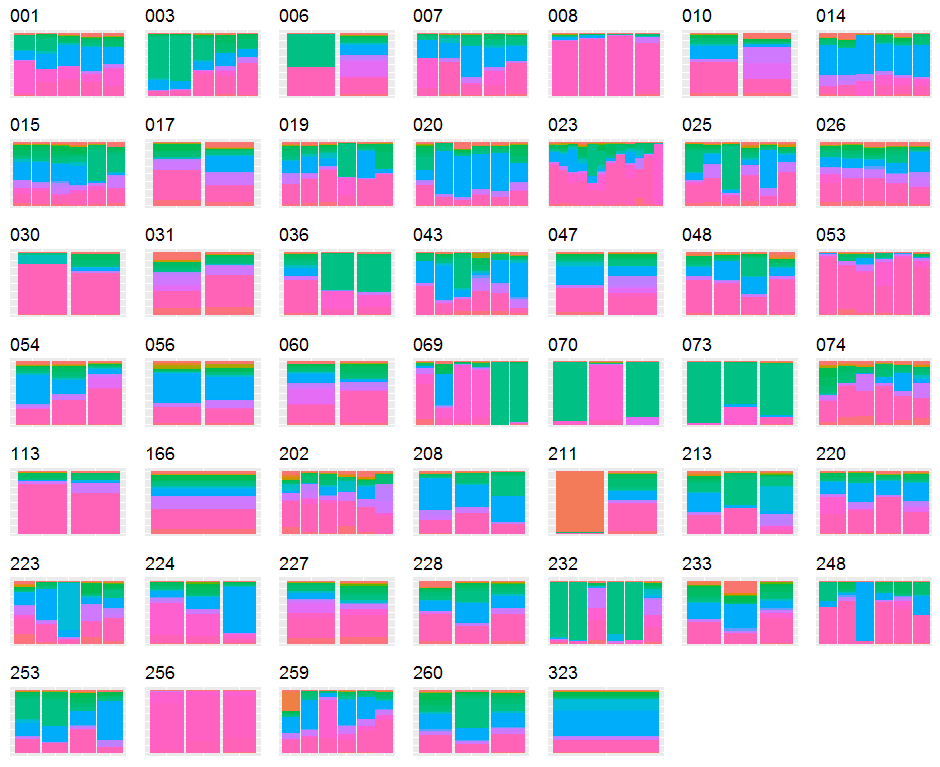
\includegraphics[scale=0.70]{img/enfin_barplot_genus_norm.png}\hfill
\end{center}
\caption{Évolution des abondances par genre}
\label{plotabundancegenre}
\end{figure}

\begin{figure}
\begin{center}
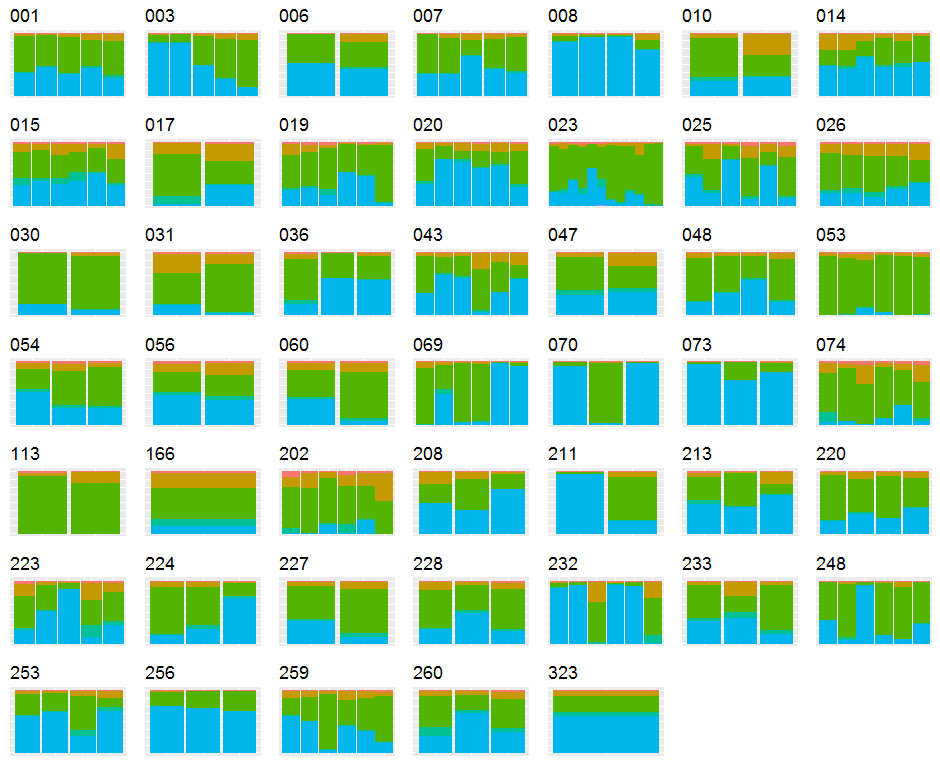
\includegraphics[scale=0.70]{img/enfin_barplot_phylum_norm.png}\hfill
\end{center}
\caption{Évolution des abondances par phylum}
\label{plotabundancephylum}
\end{figure}


\begin{figure}
\begin{center}
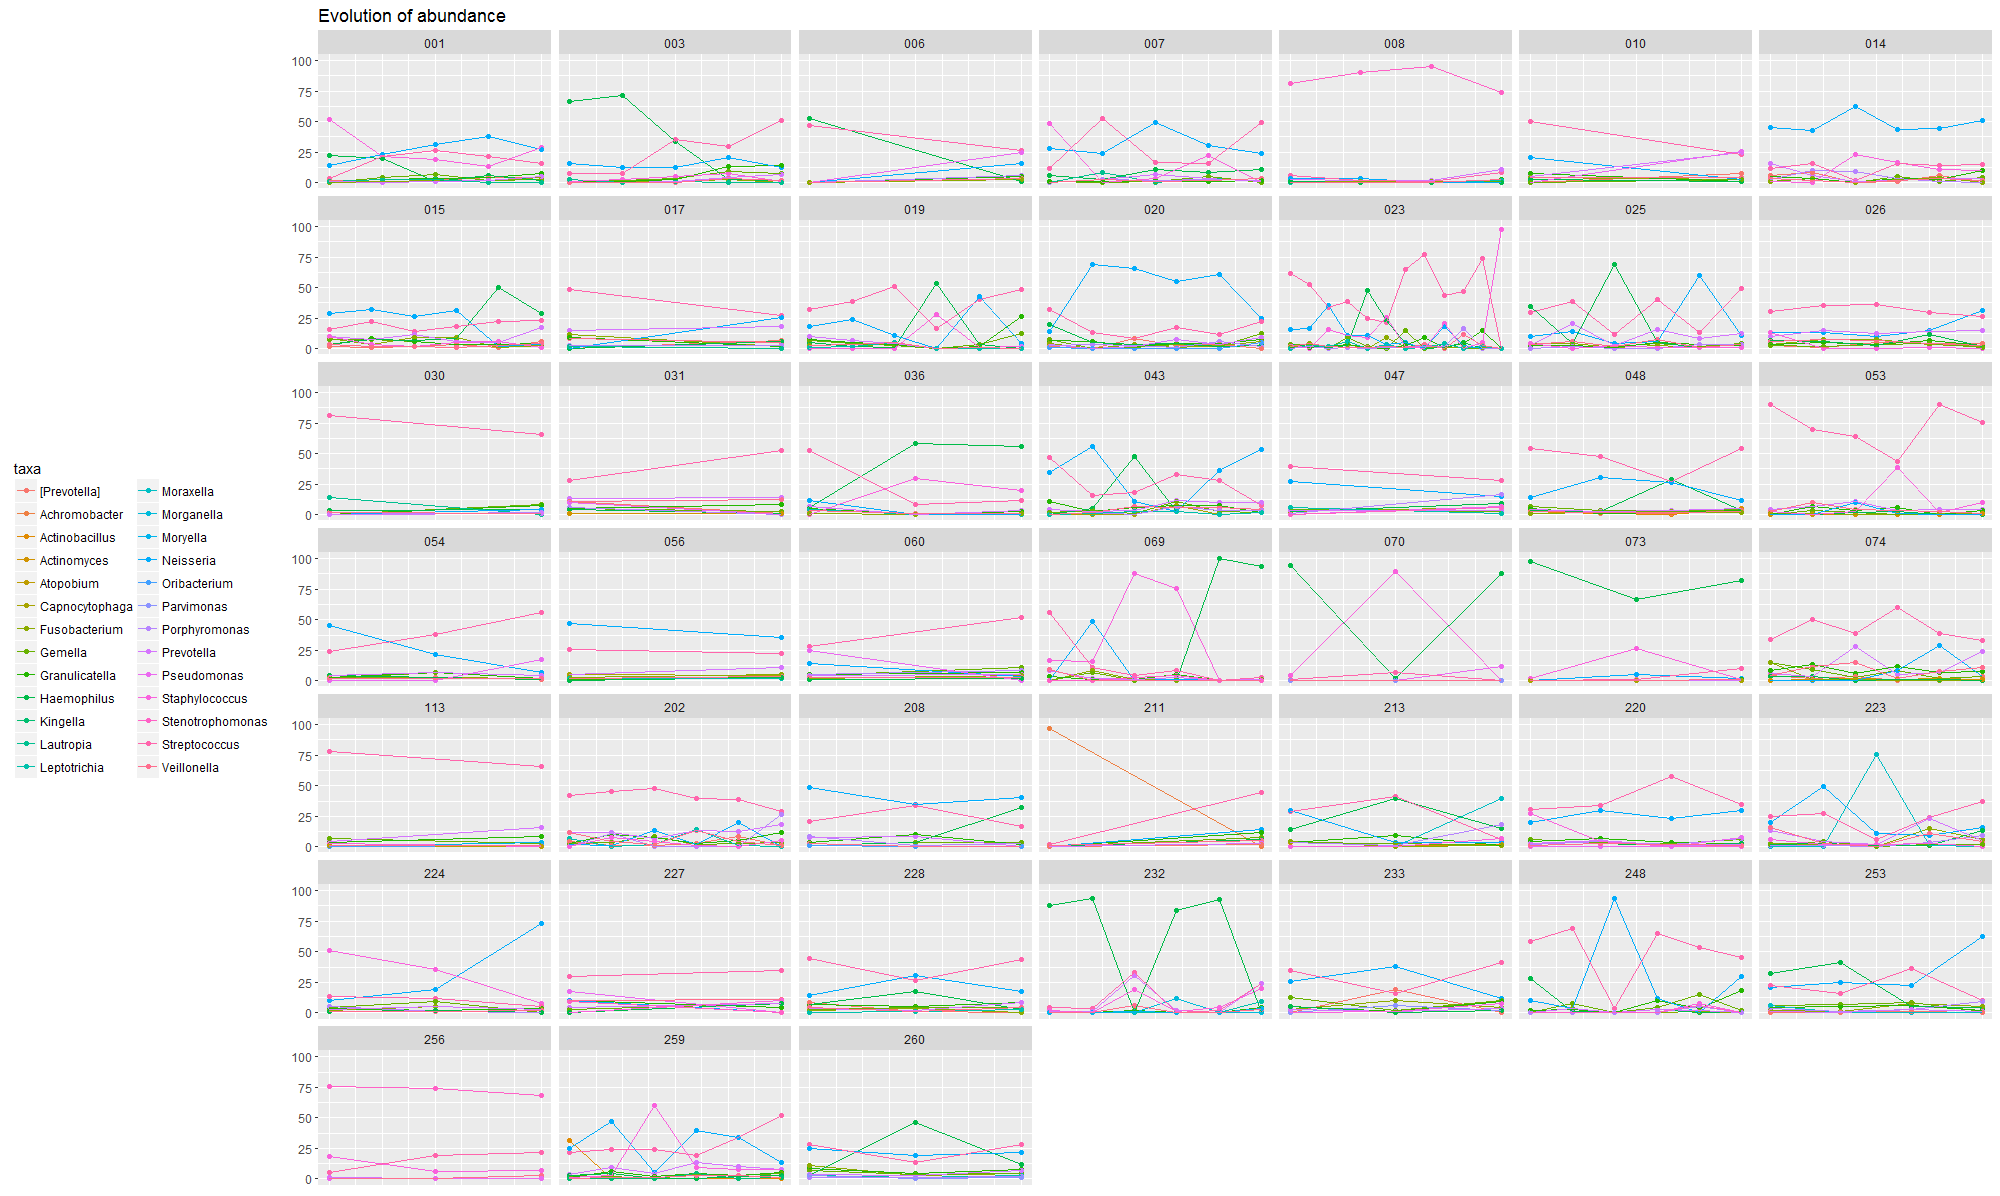
\includegraphics[scale=0.50,angle=90]{img/evolution_abundance.png}\hfill
\end{center}
\caption{Évolution des abondances par genre}
\label{plotabundancecurve}
\end{figure}


\begin{figure}
\begin{center}
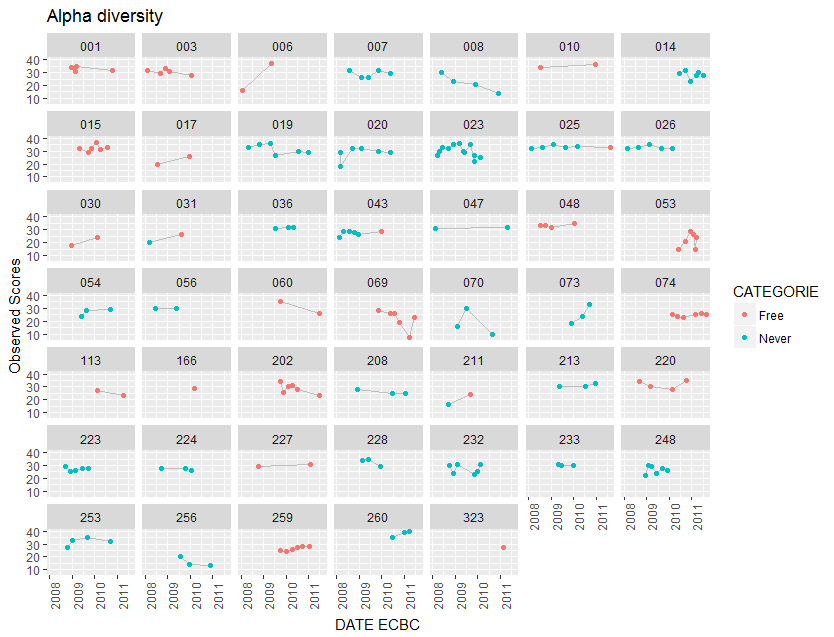
\includegraphics[scale=0.80]{img/alpha_observed.png}\hfill
\end{center}
\caption{Évolution du nombre d'espèces par patient en fonction du temps}
\label{alphaObs}
\end{figure}


\begin{figure}
\begin{center}
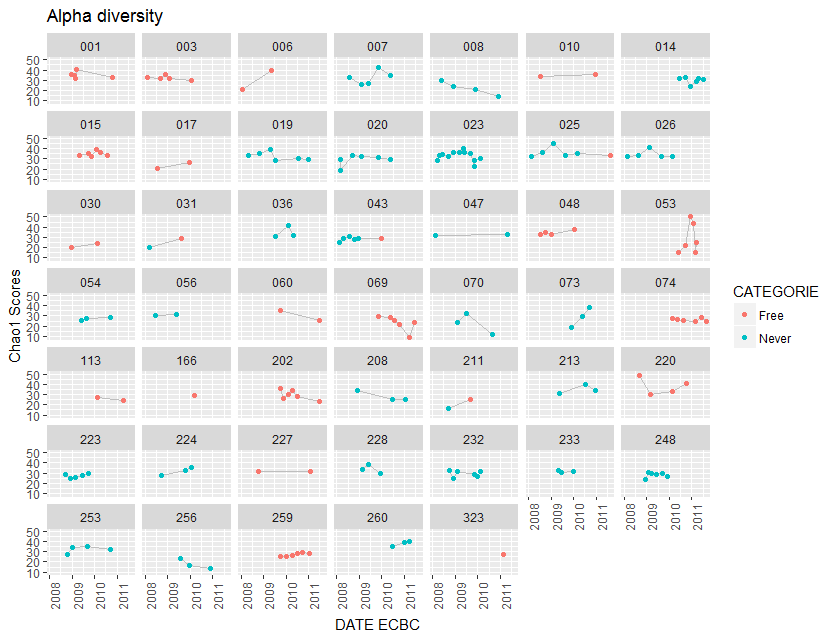
\includegraphics[scale=0.80]{img/alpha_chao1.png}\hfill
\end{center}
\caption{Évolution de l'indice de Chao1 par patient en fonction du temps}
\label{alphaChao1}
\end{figure}

\begin{figure}
\begin{center}
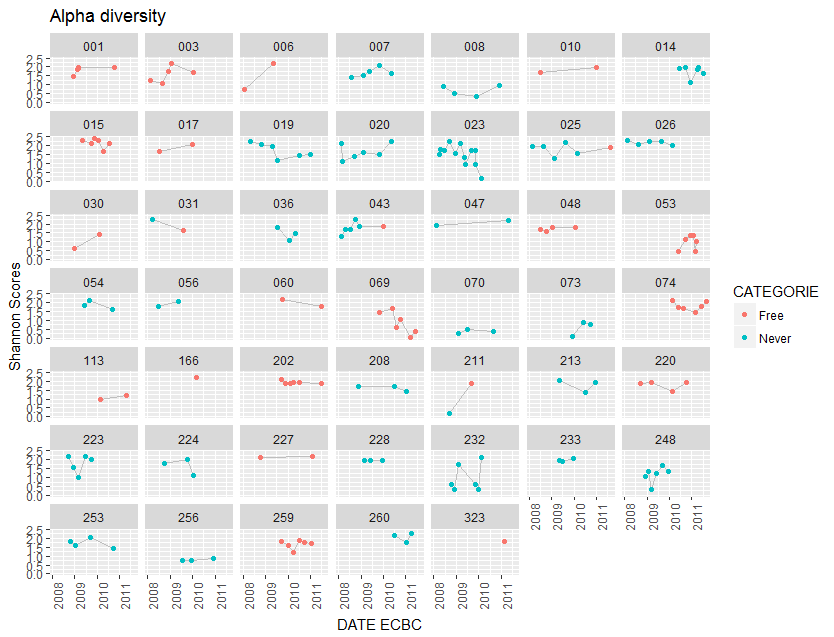
\includegraphics[scale=0.80]{img/alpha_shannon.png}\hfill
\end{center}
\caption{Évolution de l'indice de Shanon par patient en fonction du temps}
\label{alphaShannon}
\end{figure}



%%file:///home/sacha/T%C3%A9l%C3%A9chargements/%10.1183@13993003.02086-2016.pdf
%In addition, studies characterising the airway microbiome following %antibiotic treatment have shown a
%remarkable resistance of bacterial communities to change over time in these %patients [57, 59, 60];
%antibiotic treatments primarily result in a reduction in bacterial %diversity, but this effect disappears after
%some weeks, with the recovery of the previous microbial composition [57]

\newpage


\bibliographystyle{ieeetr}
\bibliography{biblio}

\end{document}
